\vspace{10pt}
\section{Analysis of Design Constraints - A Case Study}\label{sec:w_and_r}

In this section, a typical ReRAM cross-point array is analyzed in detail by using our mathematical model.

\subsection{Overview}
As shown in Figure~\ref{fig:modeling}, in order to write or read a
cross-point array, proper voltages should be applied to
wordlines and bitlines. Since several potential
read/write schemes can be used to program a memory array, it is
difficult to identify the ideal scheme that meets the design constraints in terms of area, energy, and reliability. In this section, we study the effect of various schemes on cross-point size and reliability.
The constraints on array size, energy and area overheads are analyzed in the worst cases scenario. The results of this study will be a useful guide in designing a cross-point array. %can be very useful to guide the design of the cross-point array.

%Also, we assumes that the in the case of worst scenario, the ReRAM cells at the selected wordline, th
%Since it is impossible to consider all of the data pattern stored in the array,

Table~\ref{table:parameter} shows the circuit parameters of our baseline 32nm design. The data is derived from the recently published studies on ReRAM~\cite{crossbar_TED_2010}\cite{memristor:Cong}.
We study %In the following the
reliability, energy consumption, and area overheads for four different write
schemes, and discuss the sensitivities of these schemes to the data
pattern of HRS and LRS ReRAM cells and cell non-linearity.

\begin{table}[!b]
  \centering
  \scriptsize
    \scriptsize
  \caption{Parameters of the baseline Cross-Point Array}\label{table:parameter}
  \vspace{-5pt}
%  \begin{tabular}{|cccccp{3.5cm}|}
  \begin{tabular}{c|c|c}
    \hline    \hline
    % after \\: \hline or \cline{col1-col2} \cline{col3-col4} ...
    \textbf{Metric} & \textbf{Description} & \textbf{Values} \\
    \hline
    \textbf{$S_{cell}$} & Cell Size & \textbf{$4F^2$} \\
    \textbf{$R_l$} &  Interconnection Resistance&\textbf{$1.25\Omega$} \\
    \textbf{$V_{RESET}$} & Threshold voltage for RESET&\textbf{$2.0V$} \\
    \textbf{$V_{SET}$} & Threshold voltage for SET&\textbf{$-2.0V$} \\
    \textbf{$V_{READ}$} & Read Voltage of Cell&\textbf{$0.5V$} \\
    \textbf{$R_{off}$} & HRS Resistance &\textbf{$500K\Omega$} \\
    \textbf{$R_{on}$} & LRS Resistance &\textbf{$10K\Omega$} \\
    \textbf{$V_{W}(R)$} & Wordline Voltage during Read &\textbf{$0.4V$} \\
    \textbf{$V_{W}(W)$} & Wordline Voltage during Write  &\textbf{$\pm2V$} \\
    \textbf{$V_{W}(H)$} & Half Selected wordline Voltage &\textbf{$1V$} \\
    \textbf{$V_{B}(R)$} & Bitline Voltage during Read  &\textbf{$0V$} \\
    \textbf{$V_{B}(W)$} & Bitline Voltage during Write  &\textbf{$0V$} \\
    \textbf{$V_{B}(H)$} & Half Selected bitline Voltage &\textbf{$1V$} \\
    \textbf{$M$} & Number of wordlines &\textbf{$64$} \\
    \textbf{$N$} & Number of bitline &\textbf{$64$} \\
    \hline
  \end{tabular}
  \vspace{-10pt}
\end{table}

Although the goal of a read operation is different from a write operations, both of them are realized by fully biasing the selected cell and floating (or half biasing) unselected cells. Thus, the coefficient matrix $A$ and the constant vector $C$ are very similar for both. In addition, their energy consumption and area overhead will also have a similar trend. In the next section,  we first study the writing operation comprehensively.  After that, for read operation, we mainly focus on the read margin analysis since it is unique to reads.

\subsection{Write Operation}
To write a ReRAM cell, an external voltage is applied across the cell for a certain duration. Intuitively, there are four possible schemes for the write operation:
\begin{enumerate}
  \item According to the location of a selected cell, activate one wordline and one bitline and leave all of other lines floating (FWFB shemes).
  \item Activate the selected wordline and bitline. Leave all the unselected wordlines floating and half bias the unselected bitlines (FWHB shemes).
  \item In contrast to the scheme 2, activate the selected wordline and bitline. Leave all the unselected bitlines floating and half bias the unselected wold lines (HWFB shemes).
  \item Activate the selected wordline and bitline. Then half bias all other wordlines and bitlines (HWHB shemes).
\end{enumerate}
Since reliability, energy consumption, and area overheads for these
schemes are different, we address these problems
separately and finally combine all constraints to provide design
guidelines for write operations.

\vspace{6pt} \emph{Reliable Write Operation.} \vspace{6pt}

Write reliability is a serious concern in cross-point arrays. In an ideal condition, the resistance of wires and the sneak currents in unselected cells are negligible. In such a scenario, all the write schemes discussed above will make sure that the write voltage $V_W(W)-V_B(W)$ is fully applied across the specified cell. However, in reality, both wire resistance and sneak current are non-trivial. Hence, the operation of cross-point array will vary based on the data pattern stored in ReRAM cells.
A write is considered reliable if it modifies the content of the selected cells to the new value without disturbing other unselected cells.
%A reliable write operation can be defined as: switching the selected cells into required states without disturbing the states of unselected cells.
There are two potential problems with writes: \emph{write failure}, an unsuccessful write on selected cell, and \emph{write disturbance}, an undesirable write on unselected cell. It is necessary to ensure that a write scheme guarantees reliable operation even in the worst case (w.r.t the location of cells to written and pattern stored in the cross-point array). Otherwise, after several unreliable write operations, the data stored in the cross-point array will become unpredictable.

We first use an example to show the problem with FWFB scheme, which may result in severe write disturbance.
Figure~\ref{fig:FWFR} shows the voltage drop across each ReRAM cell of a $64 \times 64$ cross-point array. In this example, in order to write the cell at the cross point of the $32^{nd}$ wordline and the $32^{nd}$ bitline, the selected wordline and bitline are biased at 2V and 0V, respectively. All of the other wordlines and bitlines are biased at 1V. The ReRAM cells at the selected bitline are in the HRS, while all of the other cells are in the LRS. It is clear that the voltage drop across the selected cell ($V_{32,32}$) almost has the same magnitude as the unselected cell at the same bitline, resulting the write disturbance to all of the unselected cells at the selected bitline. Actually, for a $M \times N$ matrix ($M>N$), the worst case voltage drop of the unselected cell can be calculated as:
\begin{equation}\label{worst_FWFB}
V_{worst}=V_{select} \cdot [1-\frac{1}{M+(N-1)R_{off}/R_{on}}].
\end{equation}

\begin{figure}[!b]
\centering
  % Requires \usepackage{graphicx}
  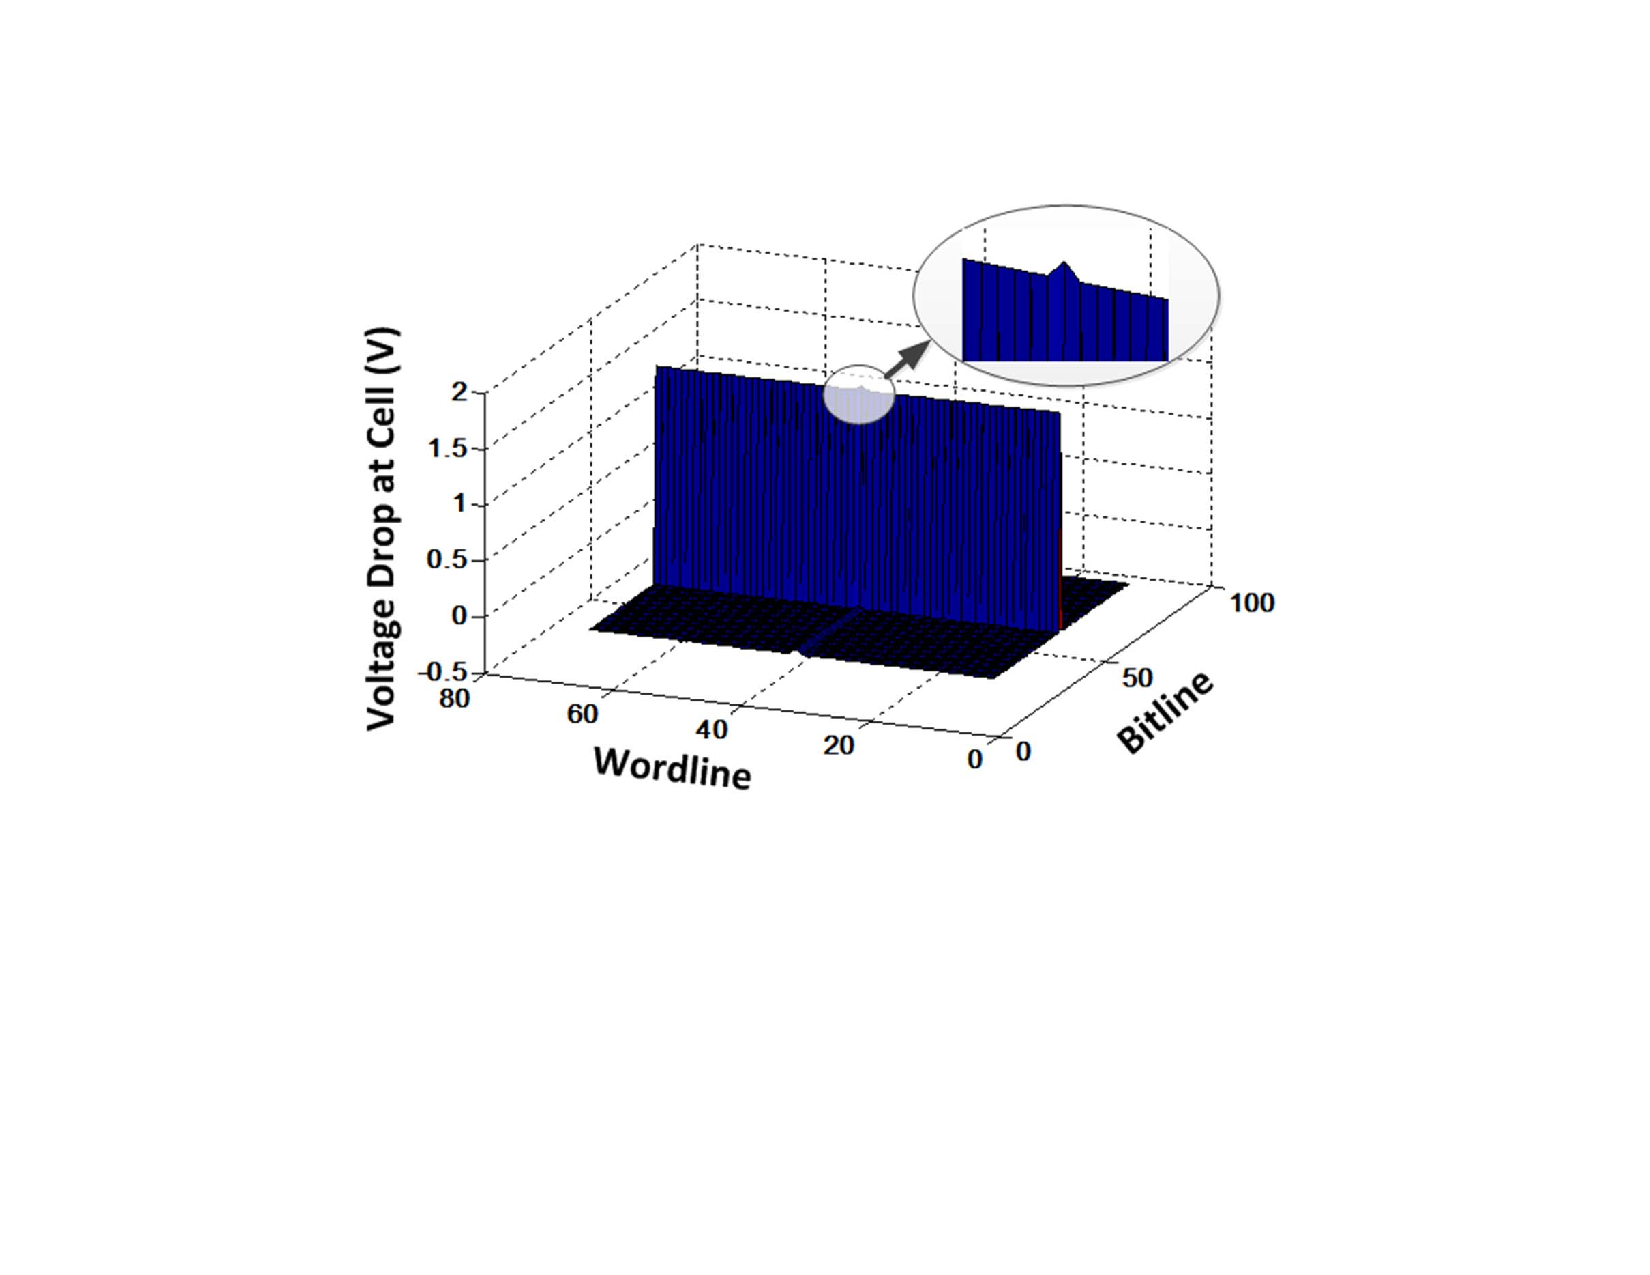
\includegraphics[width=0.4\textwidth]{./figures/FWFB_f.pdf}\\
  \caption{Write disturbance for FWFB schemes. ( $V_{W32} = 2V$, $V_{B32} = 0V$. $R_{x,32}$ at HRS, others at LRS.) }\label{fig:FWFR}
\end{figure}
Considering that the reported On-OFF resistance ratio of
ReRAM cell is always $>50$ ~\cite{ReRAM_IEDM2010_Ho,ReRAM_IEDM2010_Chien,ReRAM_IEDM2010_Lee_Diode,ReRAM_IEDM2010_Lee_Evidence,ReRAM_ISSCC2011_Sheu,ReRAM_ISSCC2011_Otsuka},
, the worst case voltage drop at the unselected cell is larger than $98\%$ of the voltage at the selected cell, making it is impossible to build a reliable cross-point structure ReRAM with the FWFB scheme. Therefore, in the following discussion, we only compare the results of FWHB, HWFB and HWHB schemes. For each of these three schemes, we can either write the cells at one wordline at the same time or only write one bit per access and separate the write operation to several arrays. In the
following discussion, we start from one bit per access write operation,
then the results of one wordline per access method are discussed.


%as long all of unselected cells in the activated wordline (or all of unselected cells in the activated bitline) are at HRS and other cells are in LRS, the voltage drop at unselected cells are mainly applied at the HRS cells at the wordline (or bitline).
%The worse case scenario for FWFB write disturbance can be defined as: all of unselected cells in the activated wordline (or all of unselected cells in the activated bitline) are at HRS and other cells are in LRS. In this case, the voltage drop at unselected cells are mainly applied at the HRS cells at the wordline (or bitline).

Write failure typically results from the voltage drop at the interconnect wires along the wordline and bitline. It has been shown that~\cite{crossbar_TED_2010}, for one bit per access write operation, the worst case voltage drop occurs when
\begin{equation}
\left\{
\begin{array}{l}
R_{M.N}=R_{on}\\
V_{WM}=V_W(W)\\
V_{BN}=V_B(W).
\end{array} \right.
\end{equation}
In order to avoid the write failure and successfully program the
selected ReRAM cell, the driven voltage should be boosted to a higher
level, making sure that the voltage across the cell exceeds the threshold
voltage even at the worst case. Figure~\ref{fig:worst_v} shows the lower bound of the driven voltage for different sizes of cross-point array. The minimum word/bitline voltage increases from 2.01~V for a $8 \times 8$ array to 4.47~V for a $128 \times 128$ cross-point array. In addition, for a  memory capability, the cross-point array can be organized with different number of wordlines and bitlines. For example, a 4K bits cross-point array can be implemented either by a $64 \times 64$ array or by a $32 \times 128$ array. In the latter case, the voltage drops along the wordline will be much more serious than along the bitline. Figure~\ref{fig:shape}
examines the voltage requirement for different array organizations with different write schemes. The result shows that from a reliability point of view, a cross-point array with same numbers of wordlines and bitlines is the best choice. Furthermore, we also notice that when the array has the same number of wordlines and bitlines, FWFB, HWFB and FWHB schemes have the same minimum driven voltage.

%Clearly, the magnitude of the voltage drop increases with the array size and the resistance of interconnect wires.

\begin{figure}%[!hb]
\centering
  % Requires \usepackage{graphicx}
  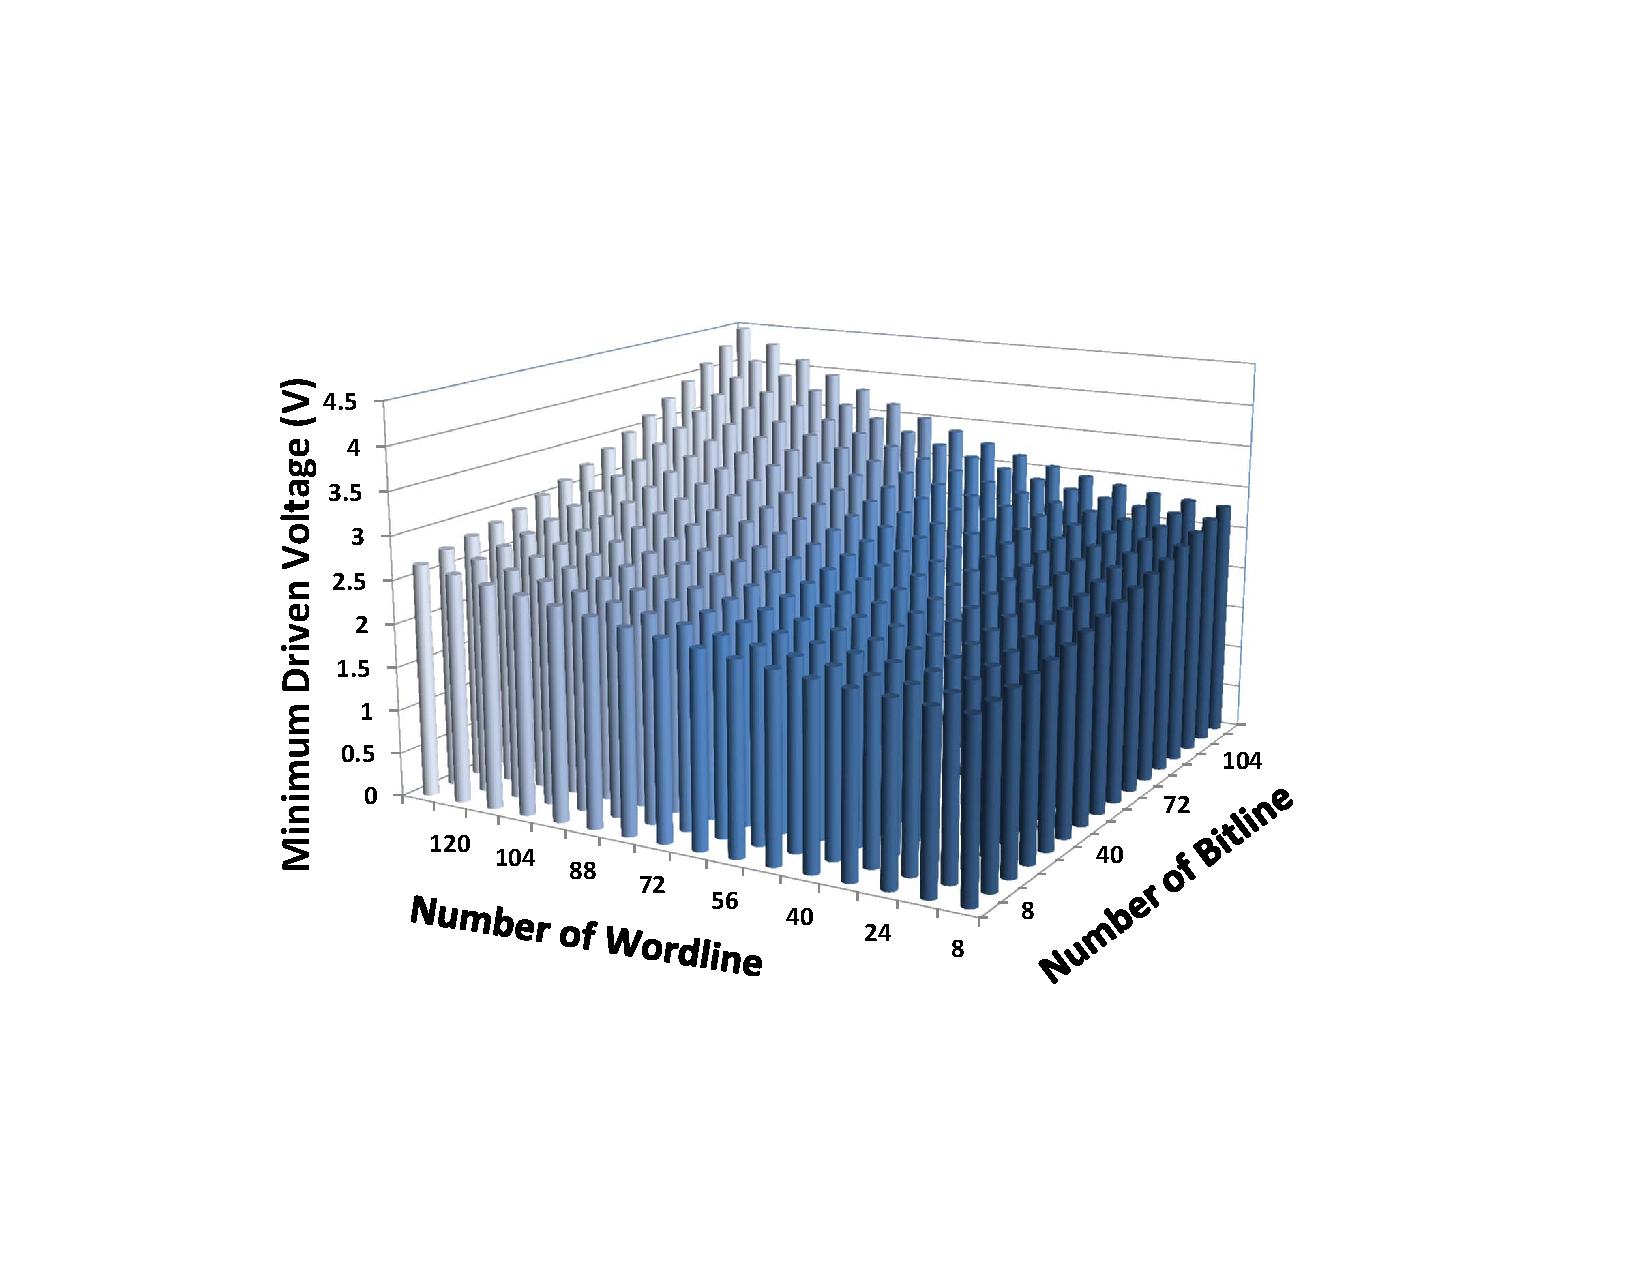
\includegraphics[width=0.4\textwidth]{./figures/worst_v_f.pdf}\\
  \caption{Write voltage requirement (Threshold voltage = 2V). }\label{fig:worst_v}
  \vspace{-10pt}
\end{figure}


\begin{figure}%[!t]
\centering
  % Requires \usepackage{graphicx}
  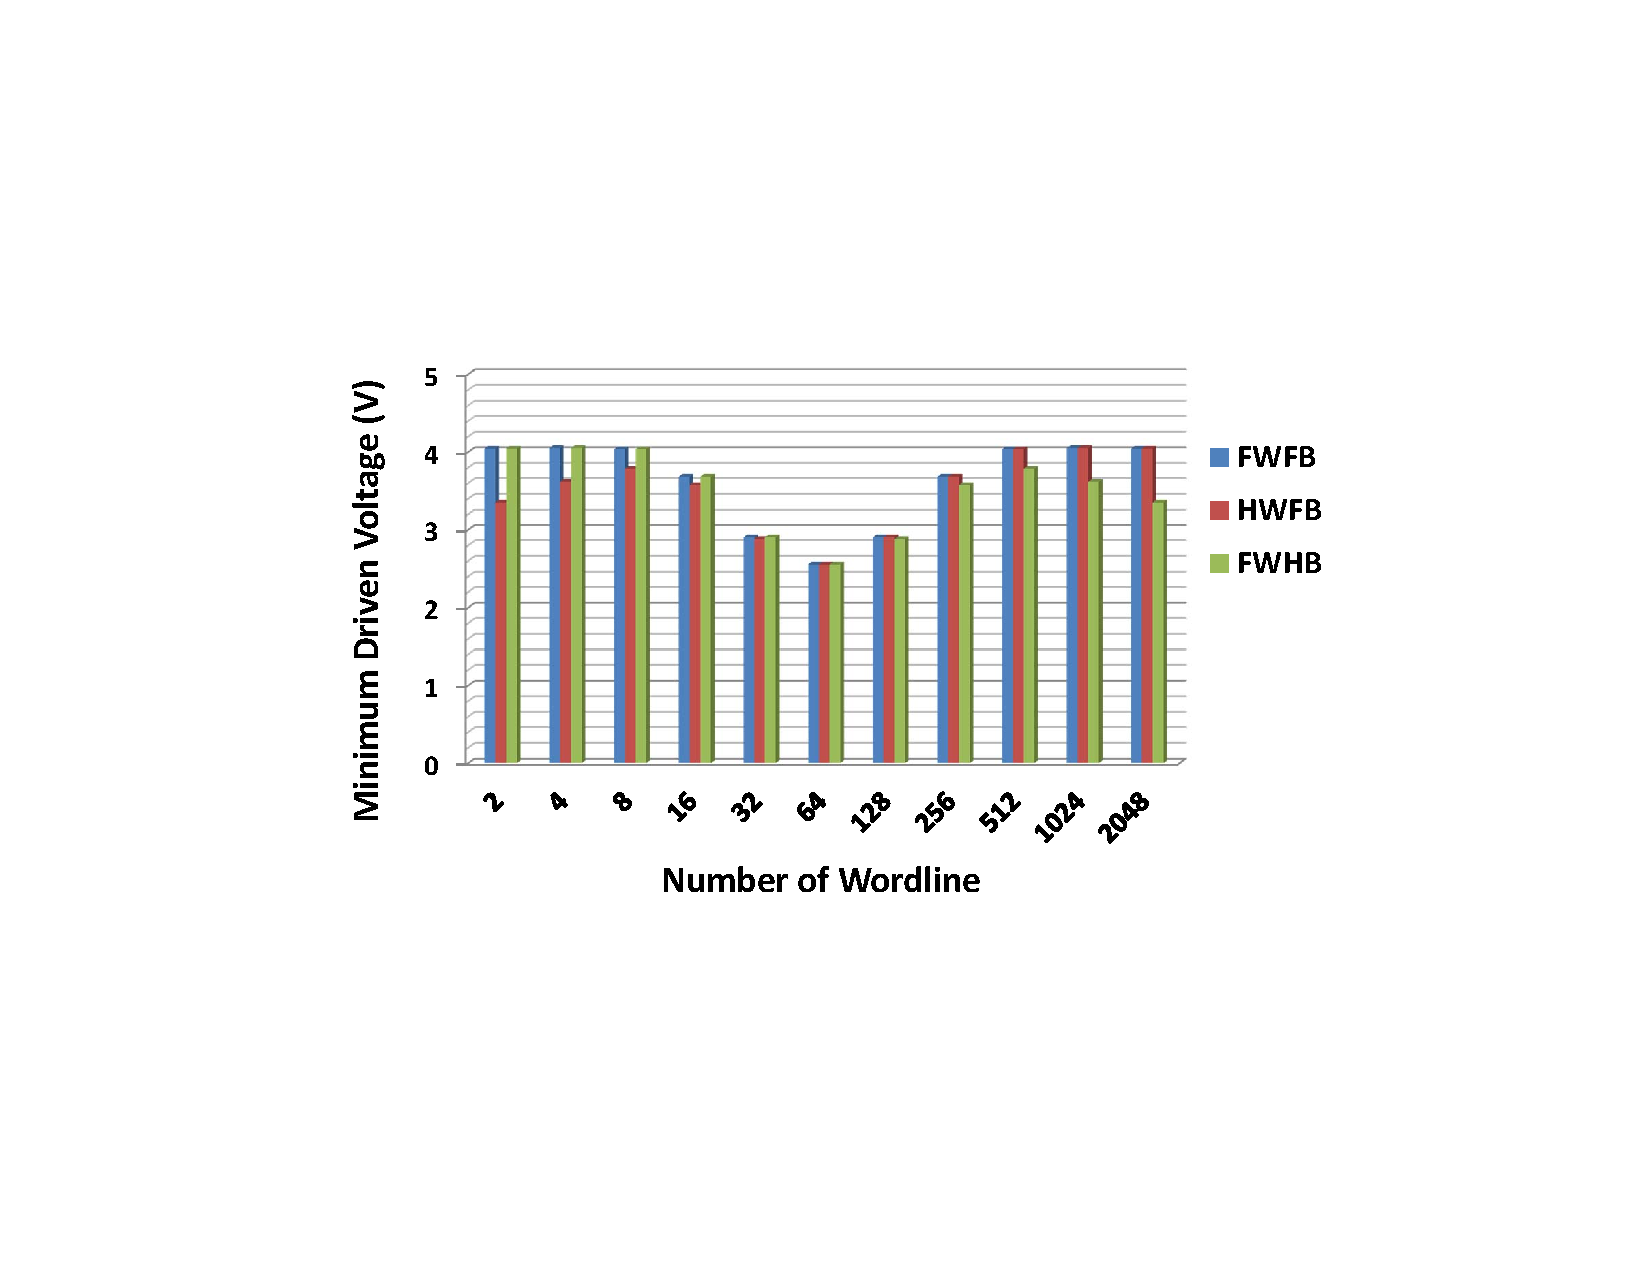
\includegraphics[width=0.45\textwidth]{./figures/shape_f.pdf}\\
  \caption{Write voltage requirement with different memory shape. (Array capacity = 4Kbits, Activated wordline voltage = 2V, Activated bitline voltage = 0V.)}\label{fig:shape_f}
    \vspace{-10pt}
\end{figure}

However, boosting the driven voltage also introduces other potential problems for the array. In particular, increasing the driven voltage also increases the voltage applied at unselected cells. Therefore, a
write disturbance may occur when the voltage applied at an unselected cell exceeds the threshold voltage for SET or RESET operation. Figure~\ref{fig:half} shows the maximum voltage applied at
unselected cells with the minimum driven voltage, which is determined in
Figure~\ref{fig:worst_v}. Since the threshold voltage of the ReRAM cell is 2V, only array sizes with worst case voltage less than 2V are allowable. Otherwise, the array is unreliable because it can not avoid write failure and write disturbance at the same time. Therefore, Figure~\ref{fig:half} provides a hard constraint on array size, and all of the following energy and area tradeoffs should be bounded by this constraint.

\begin{figure}%[!t]
\centering
  % Requires \usepackage{graphicx}
  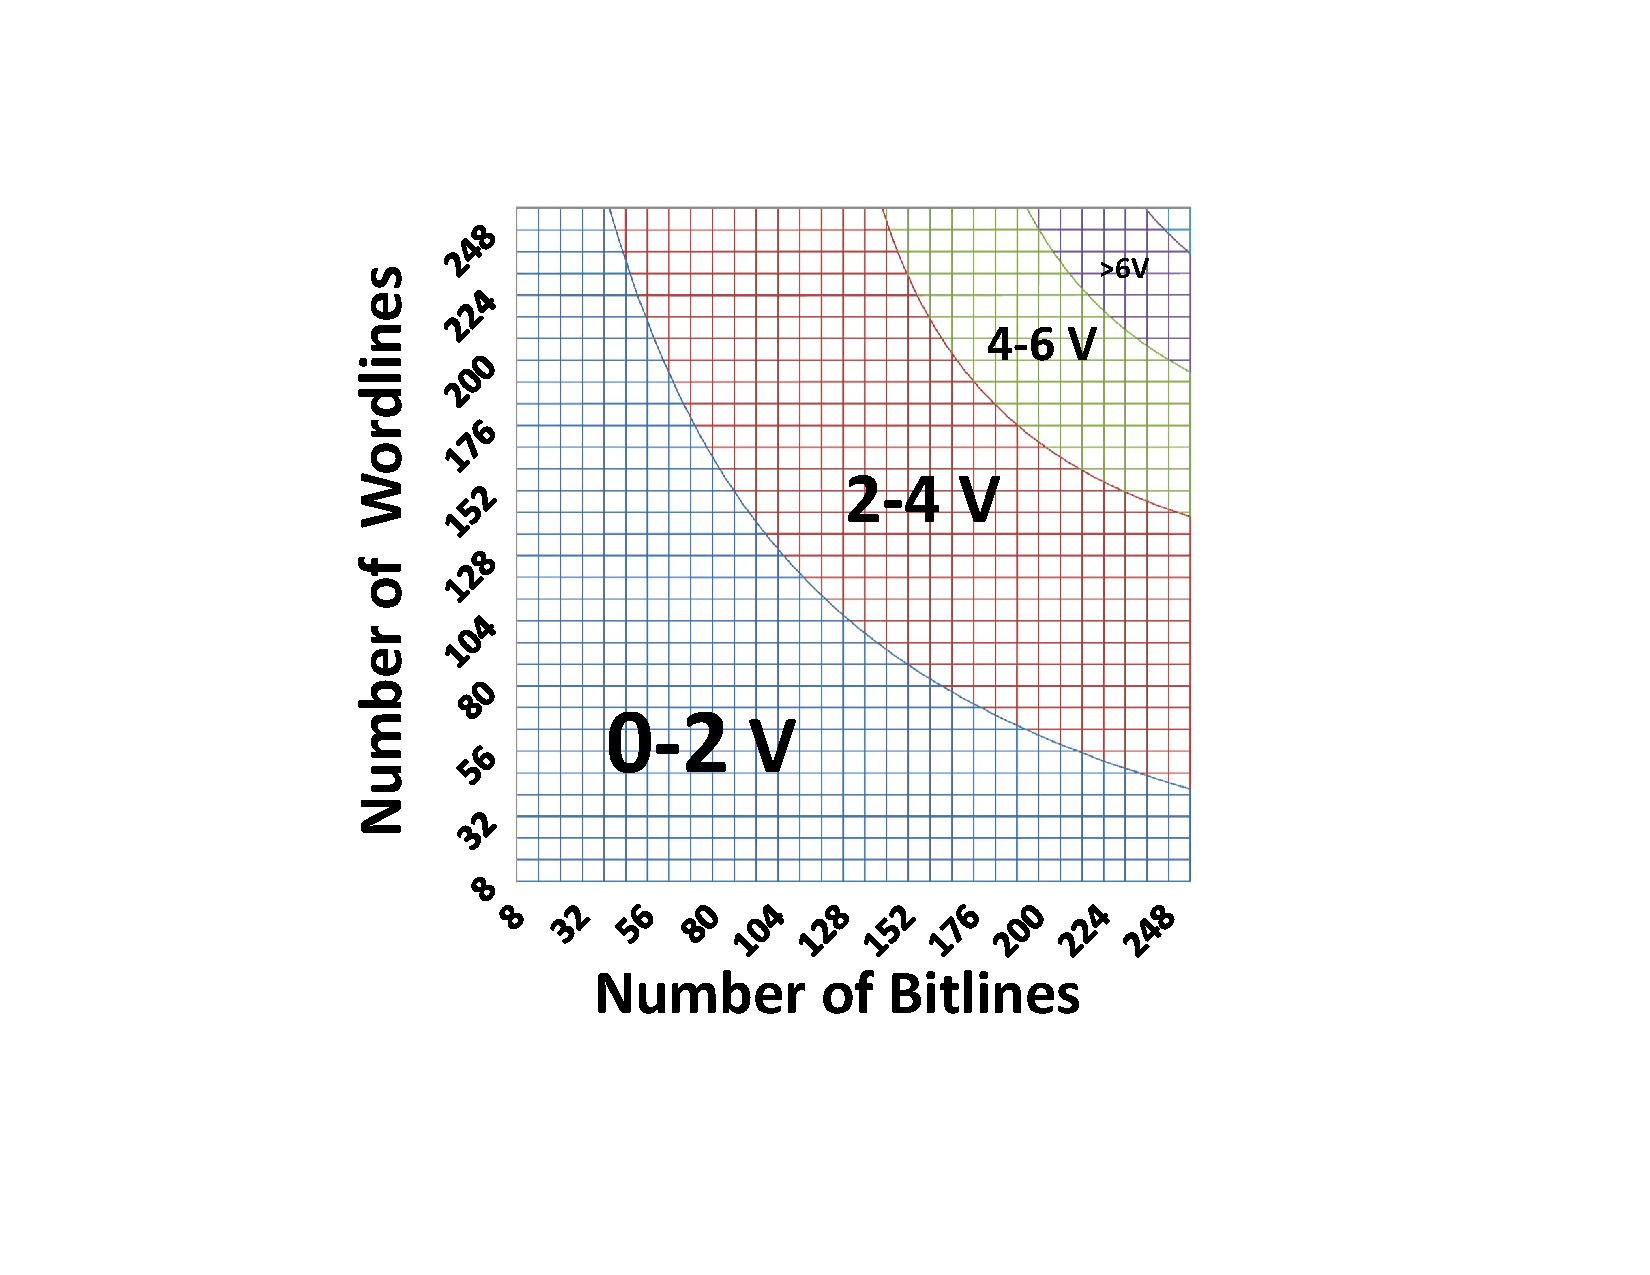
\includegraphics[width=0.28\textwidth]{./figures/Theoretical_bound_f.pdf}\\
  \caption{The maximum voltage applied at unselected cells with the minimum driven voltage.}\label{fig:half}
  \vspace{-10pt}
\end{figure}



\vspace{6pt} \emph{Energy Consumption of Write Operation.} \vspace{6pt}

The energy consumption of a write operation for a cross-point array can be calculated as:
\begin{equation}
E_{write} = E_{select} + E_{unselect} + E_{halfselect} + E_{line},
\end{equation}
where the $E_{select}$ is the energy consumed to change the state of the
selected cell, the $E_{unselect}$ and $E_{halfselect}$ are the undesired energy wasted at the half selected and unselected cells. The energy consumed by the interconnect lines are represented by $E_{line}$. Figure~\ref{fig:energy} shows the decomposed energy consumption for the cross-point array. Note that, the $E_{line}$ and $E_{halfselect}$ take a large amount of the total energy consumption. Note, the energy wasted during the write operation takes a great part of the total energy for large array sizes. For example, the undesired energy consumption for writing a $128{\times}128$ array is more than 1000 times larger than the $8{\times}8$ array. We also notice that, since the impact of sneak paths for floating schemes (FWHB and HWFB) is more serious, the energy consumed at unselected cells for floating schemes is larger than the half-biased scheme. Due to this reason, the total energy consumptions for FWHB and HWFB schemes are at least 10\% larger than that of HWHB scheme.


\begin{figure}%[!t]
\centering
  % Requires \usepackage{graphicx}
  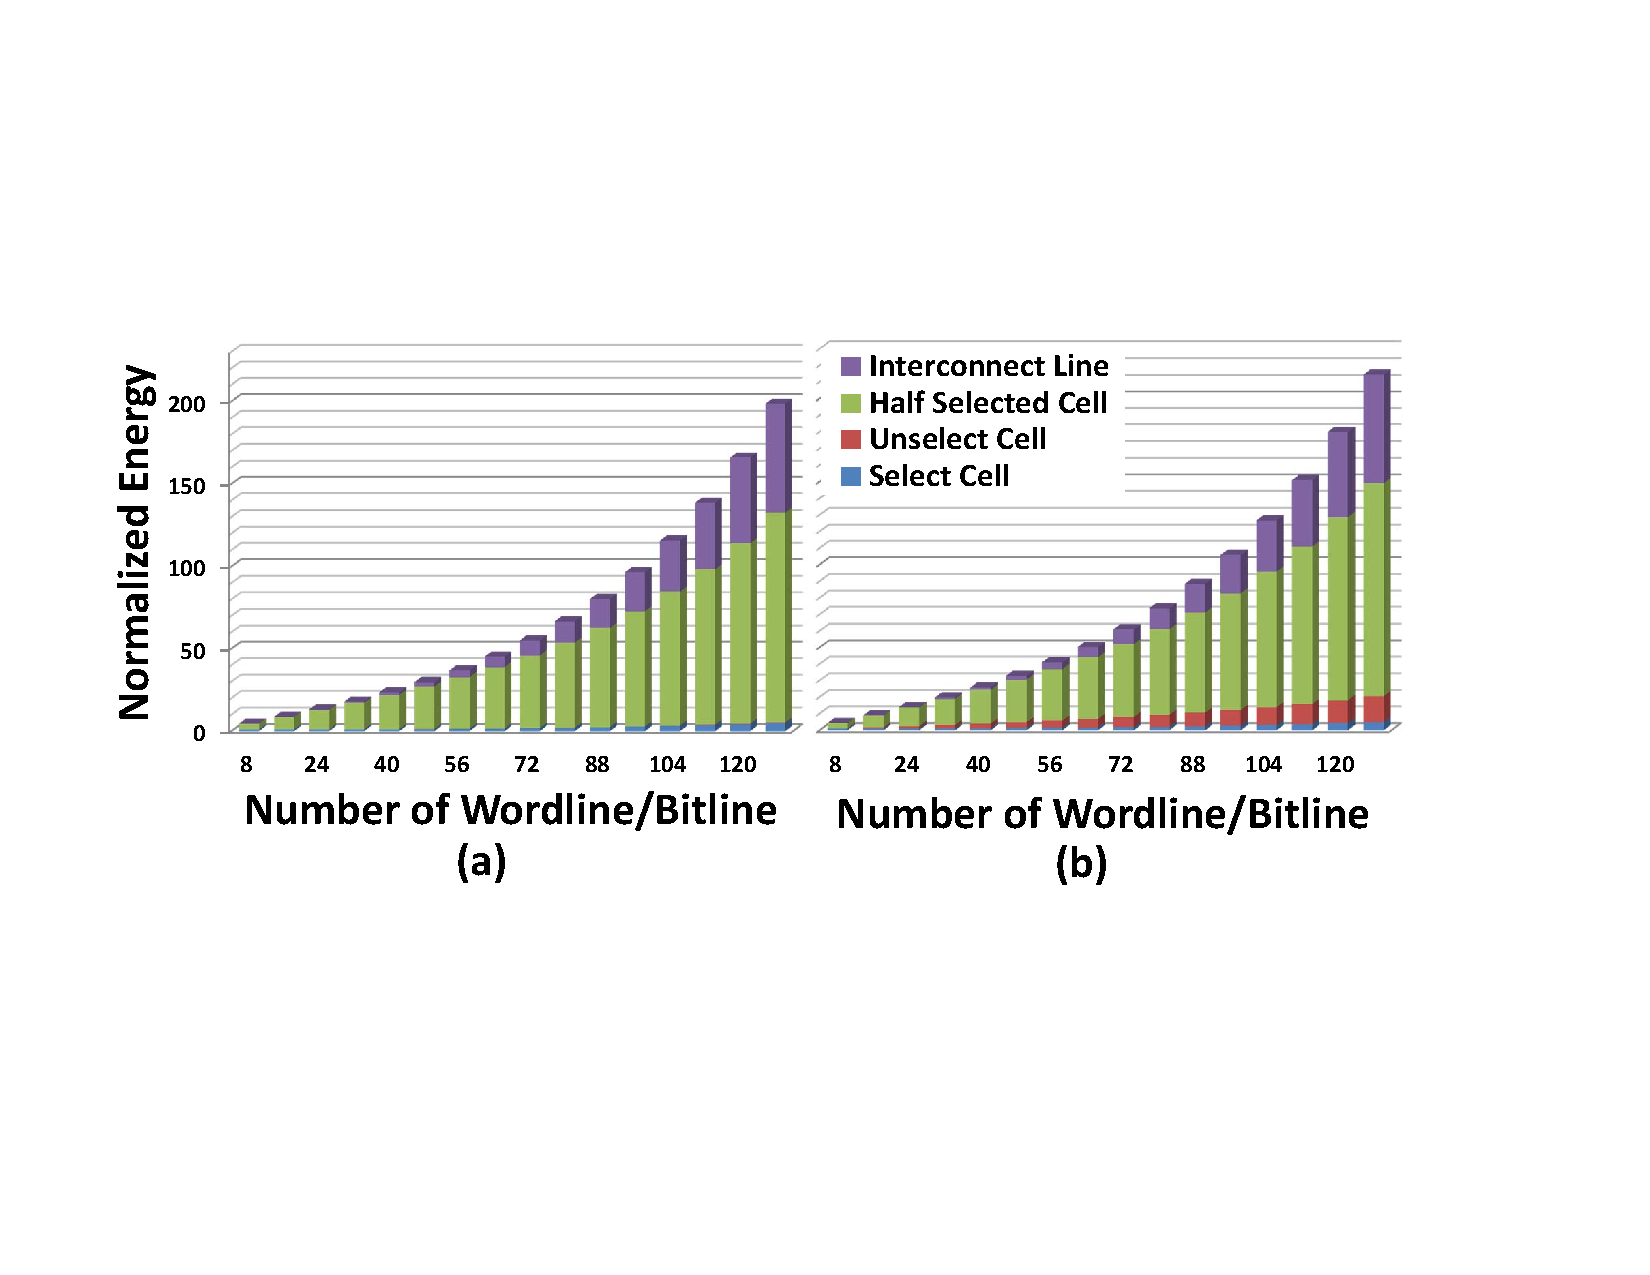
\includegraphics[width=0.5\textwidth]{./figures/energy_f.pdf}\\
  \caption{The normalized energy consumption. (a): HWHB scheme (b): FWHB and HWFB schemes.}\label{fig:energy}
    \vspace{-10pt}
\end{figure}

\vspace{6pt} \emph{Area cost of Write Operation.} \vspace{6pt}

The write operation for a $M \times N$ array requires totaly $M+N$ voltage drivers. Therefore, the average number of ReRAM cells per voltage driver can be calculated as $mn/(m+n)$. Given the array capacity of $C_{array}$, it is easy to find that the optimal array organization can be achieved when $M=N=\sqrt{C_{array}}$ and the maximum number of cells per voltage driver is: $\sqrt{C_{array}}/2$. However, the area overhead of a voltage driver is also related to its current drive capability. Figure~\ref{fig:drive_i}(a) shows the maximum write current with different ReRAM array sizes. According to the current requirement, the area of the voltage driver can be directly calculated, which will be shown in the following discussion.

%\begin{figure}%[!t]
%\centering
%  % Requires \usepackage{graphicx}
%  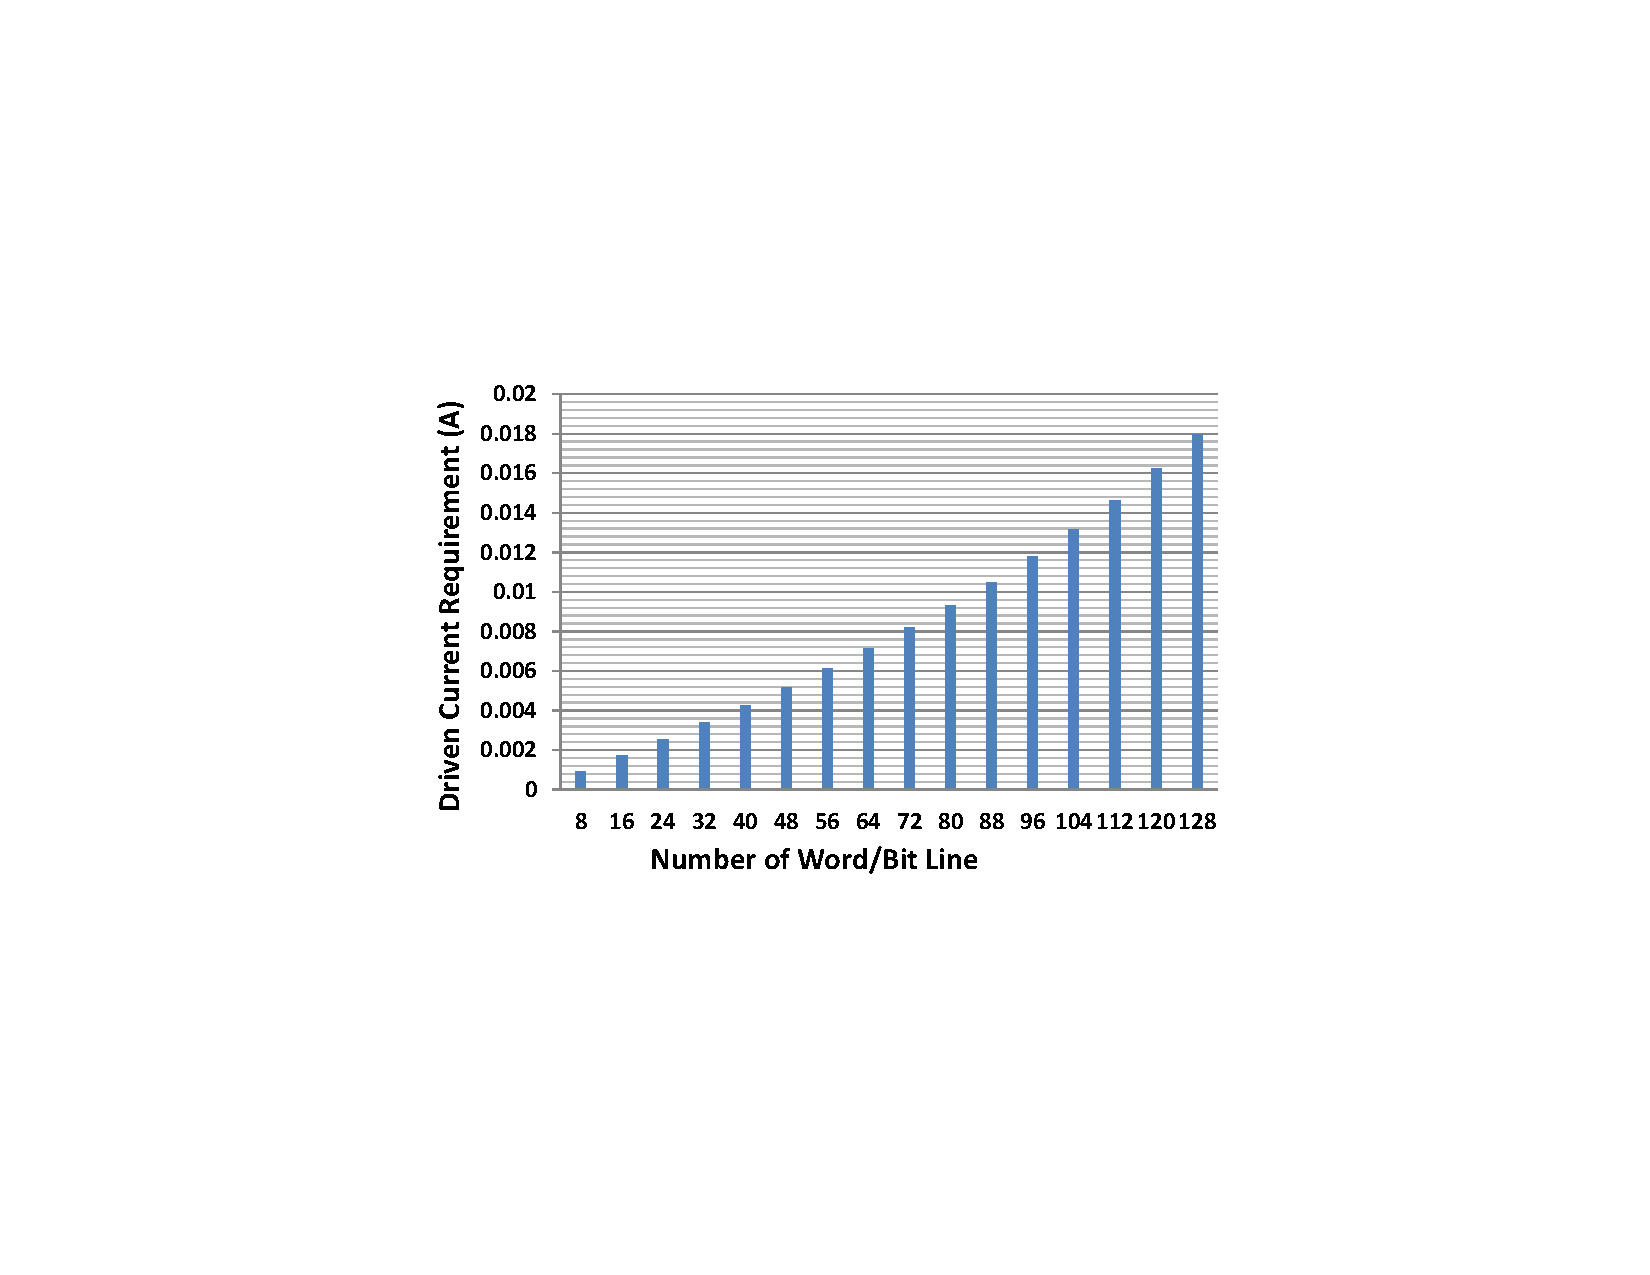
\includegraphics[width=0.4\textwidth]{./figures/w_current2.pdf}\\
%  \caption{The }\label{fig:w_current}
%\end{figure}
\begin{figure}%[!t]
\centering
  % Requires \usepackage{graphicx}
  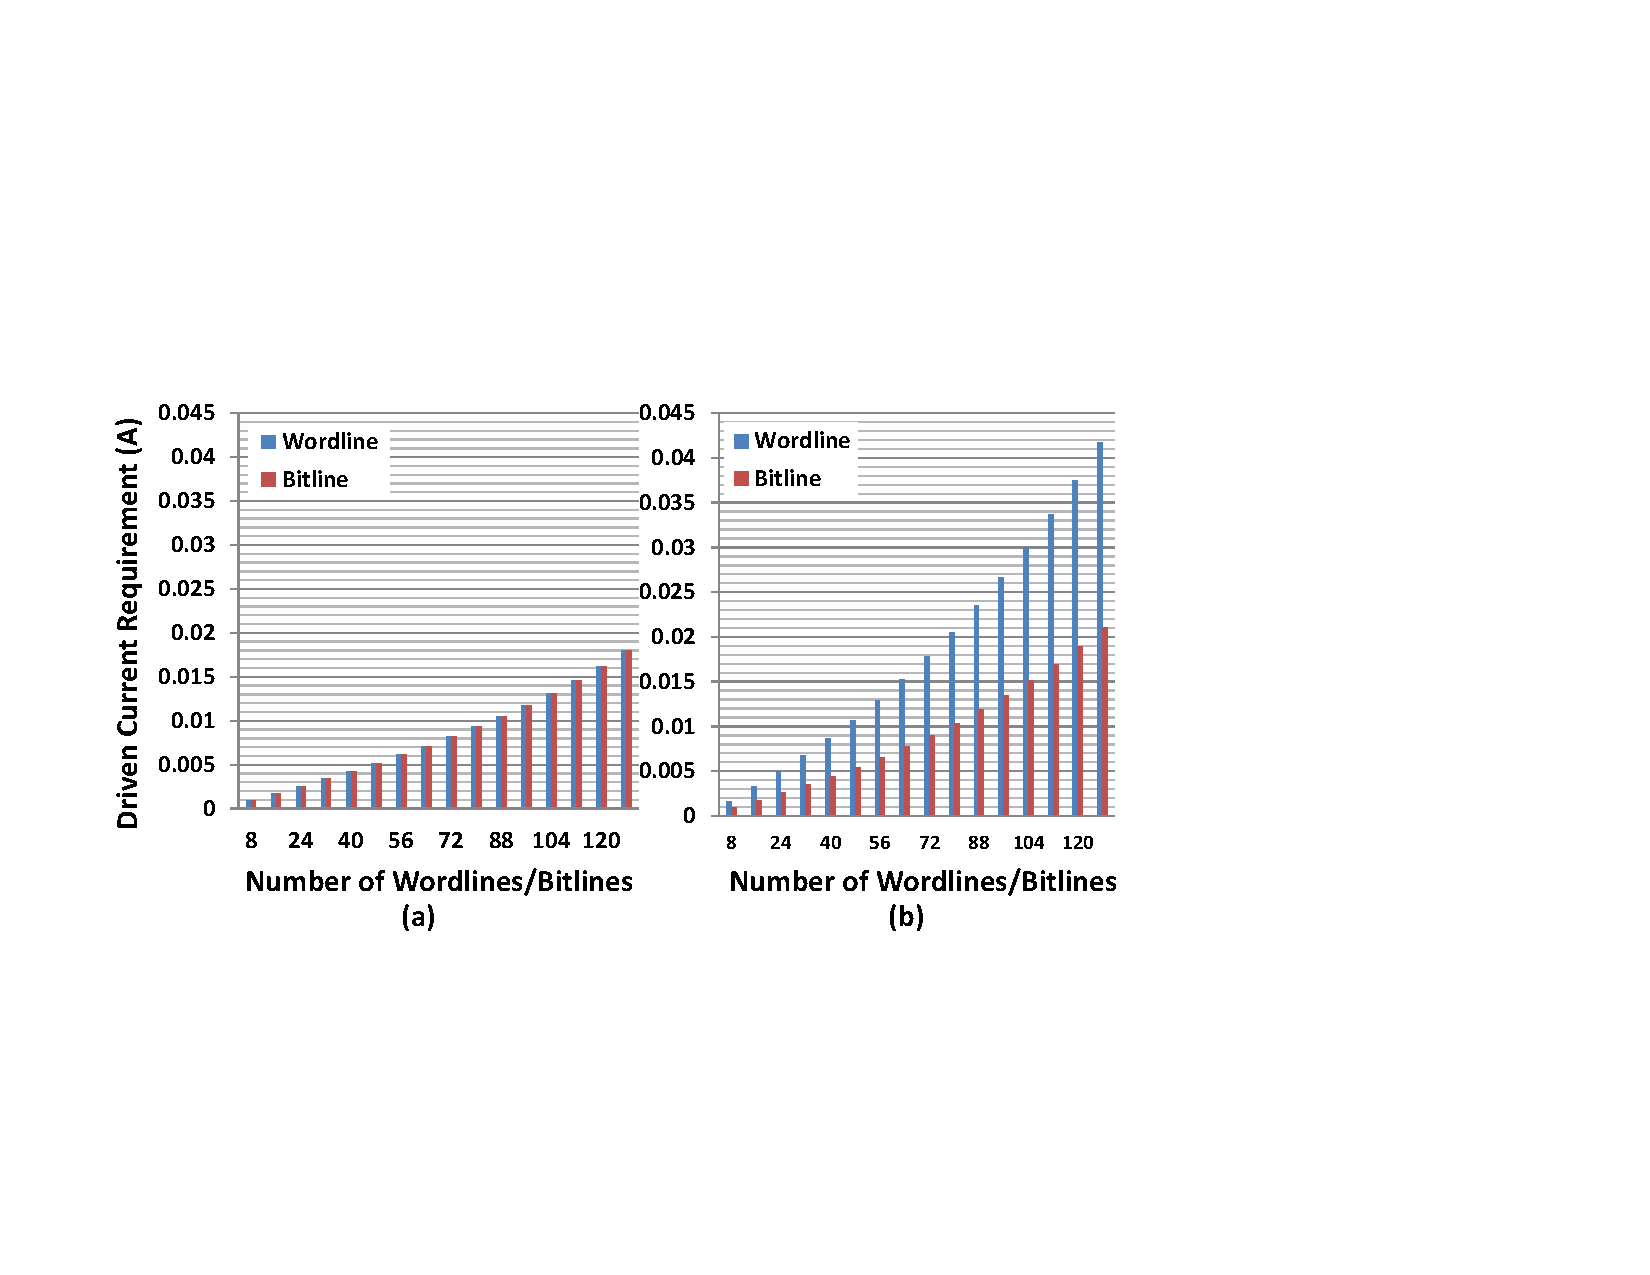
\includegraphics[width=0.5\textwidth]{./figures/drive_i_f.pdf}\\
  \caption{The driven current requirements for wordlines and bitlines. (a) One bit writing; (B) Multi bit writing.}\label{fig:drive_i}
\end{figure}


\vspace{6pt} \emph{Discussion on Multi-Bits Write Operation.} \vspace{6pt}

So far, we have only discussed the write operation with one bit per access. In this section, we consider the difference between one bit per access and one wordline per access write operations. Firstly, writing a wordline at a time will worsen the voltage drop along the wordline. Therefore, as shown in Figure~\ref{fig:reliable_region}, the reliable size of the cross-point array will be further reduced. The maximum array size reduces from $116{\times}116$ to $100{\times}100$ for HWFB and HWFB schemes.

%For the energy consumption point of view, the one wordline write operation is more efficient.

\begin{figure}%[!t]
\centering
  % Requires \usepackage{graphicx}
  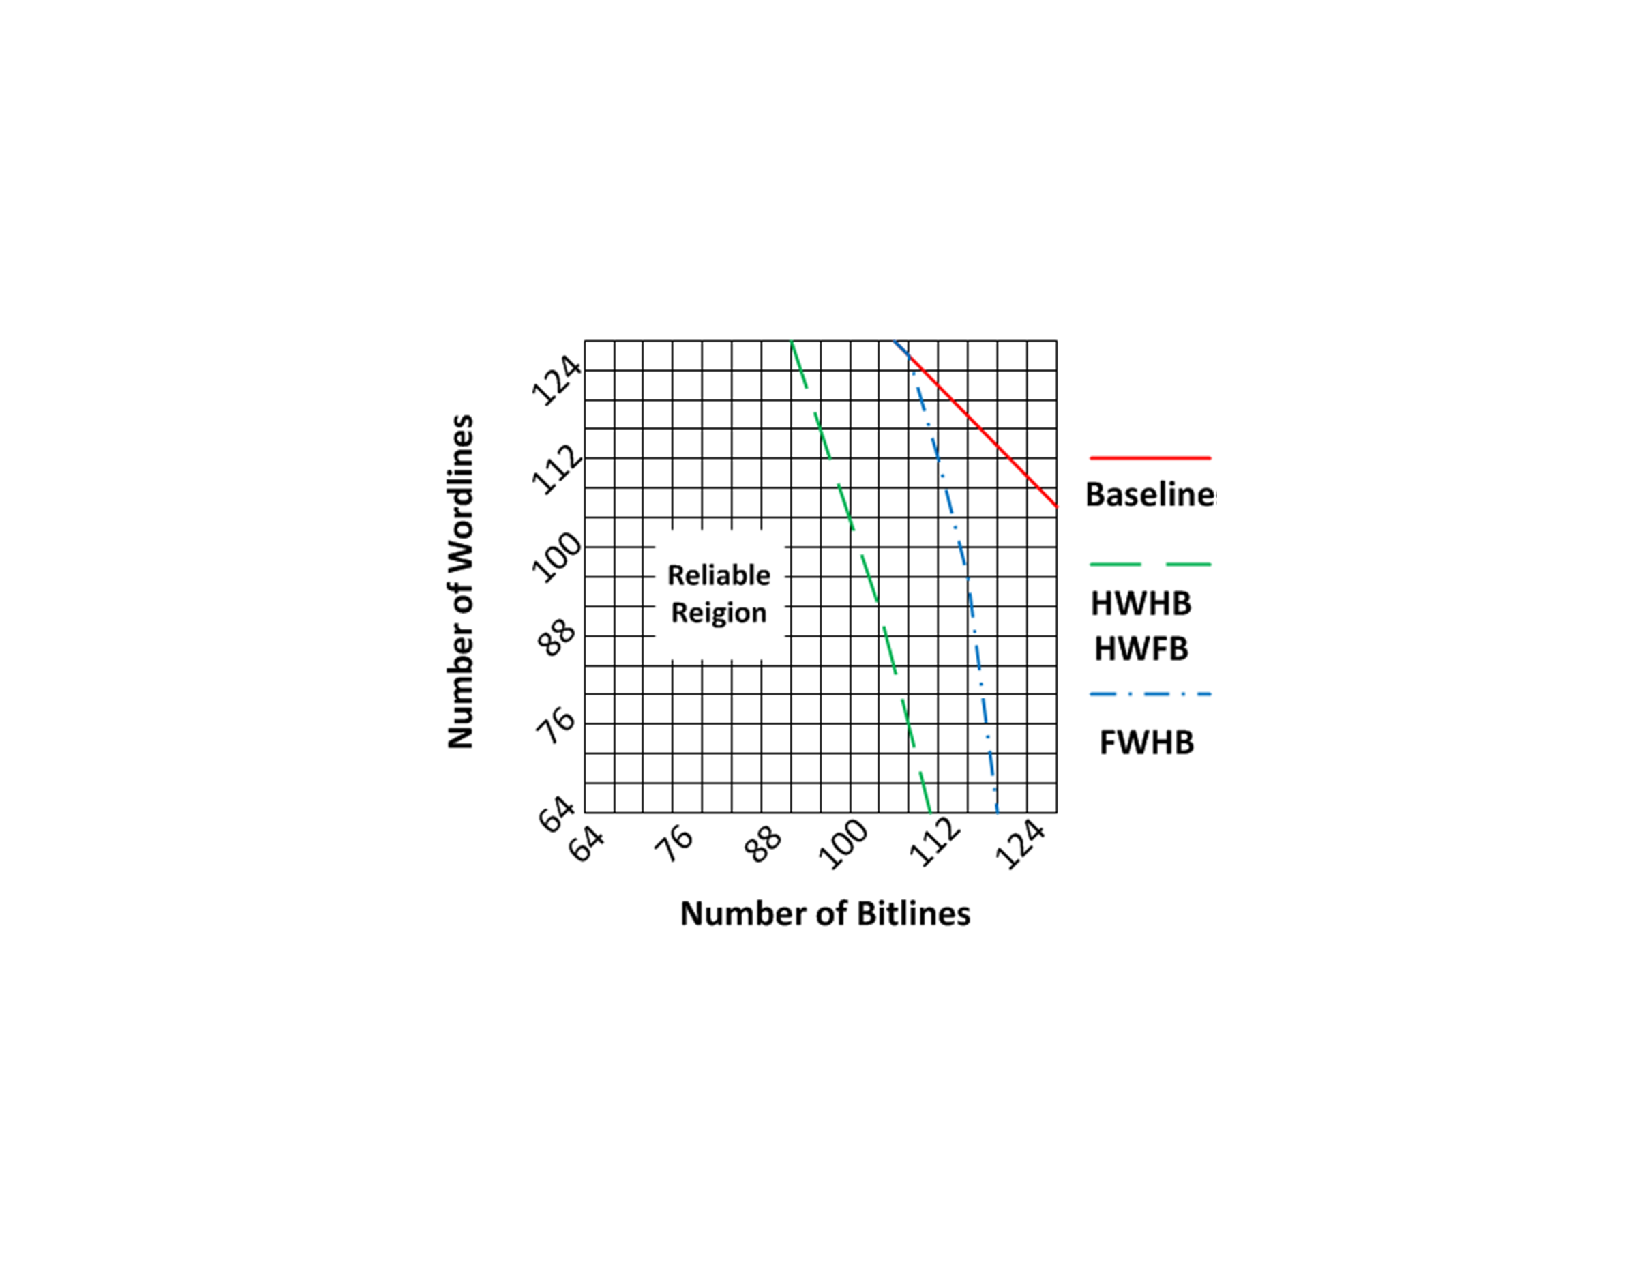
\includegraphics[width=0.4\textwidth]{./figures/multiwrite_f.pdf}\\
  \caption{The array size requirement for the cross-point array with different write schemes. (Baseline: one bit per access. HWHB, HWFB and FWHB: one wordline per access. }\label{fig:reliable_region}
    \vspace{-10pt}
\end{figure}

In order to fairly compare the energy consumption, we compare the energy-per-bit instead of the total energy. For example, in order to write a wordline with size of 128, the energy-per-bit can be calculated as:
$E_{ave}=E_{total}/128/2$. Figure~\ref{fig:multi_energy} shows the energy-per-bit of the multi-bit write operation. The energy shown in this figure is normalized to the same unit as Figure~\ref{fig:energy} for easier comparison. The results show that for large cross point array sizes, the multi-bit write operation is much more energy efficient. This is because the energy wasted at the unselected and half-selected cells are shared by multiple bits and the average energy for one each bit is therefore reduced. However, although the multi bit write operation has the advantage of lower energy consumption, the maximum current requirement for each wordline also increases. As shown in Figure~\ref{fig:drive_i}(b), the maximum driven current for each bitline is almost the same as when writing one bit, however the drive capability for each word line is almost doubled for multi-bit writing. Since the area of the voltage driver increases proportionally with its drive capability, the area overhead for multi-bit writing is about 50\% larger than for one bit writing.

\begin{figure}%[!t]
\centering
  % Requires \usepackage{graphicx}
  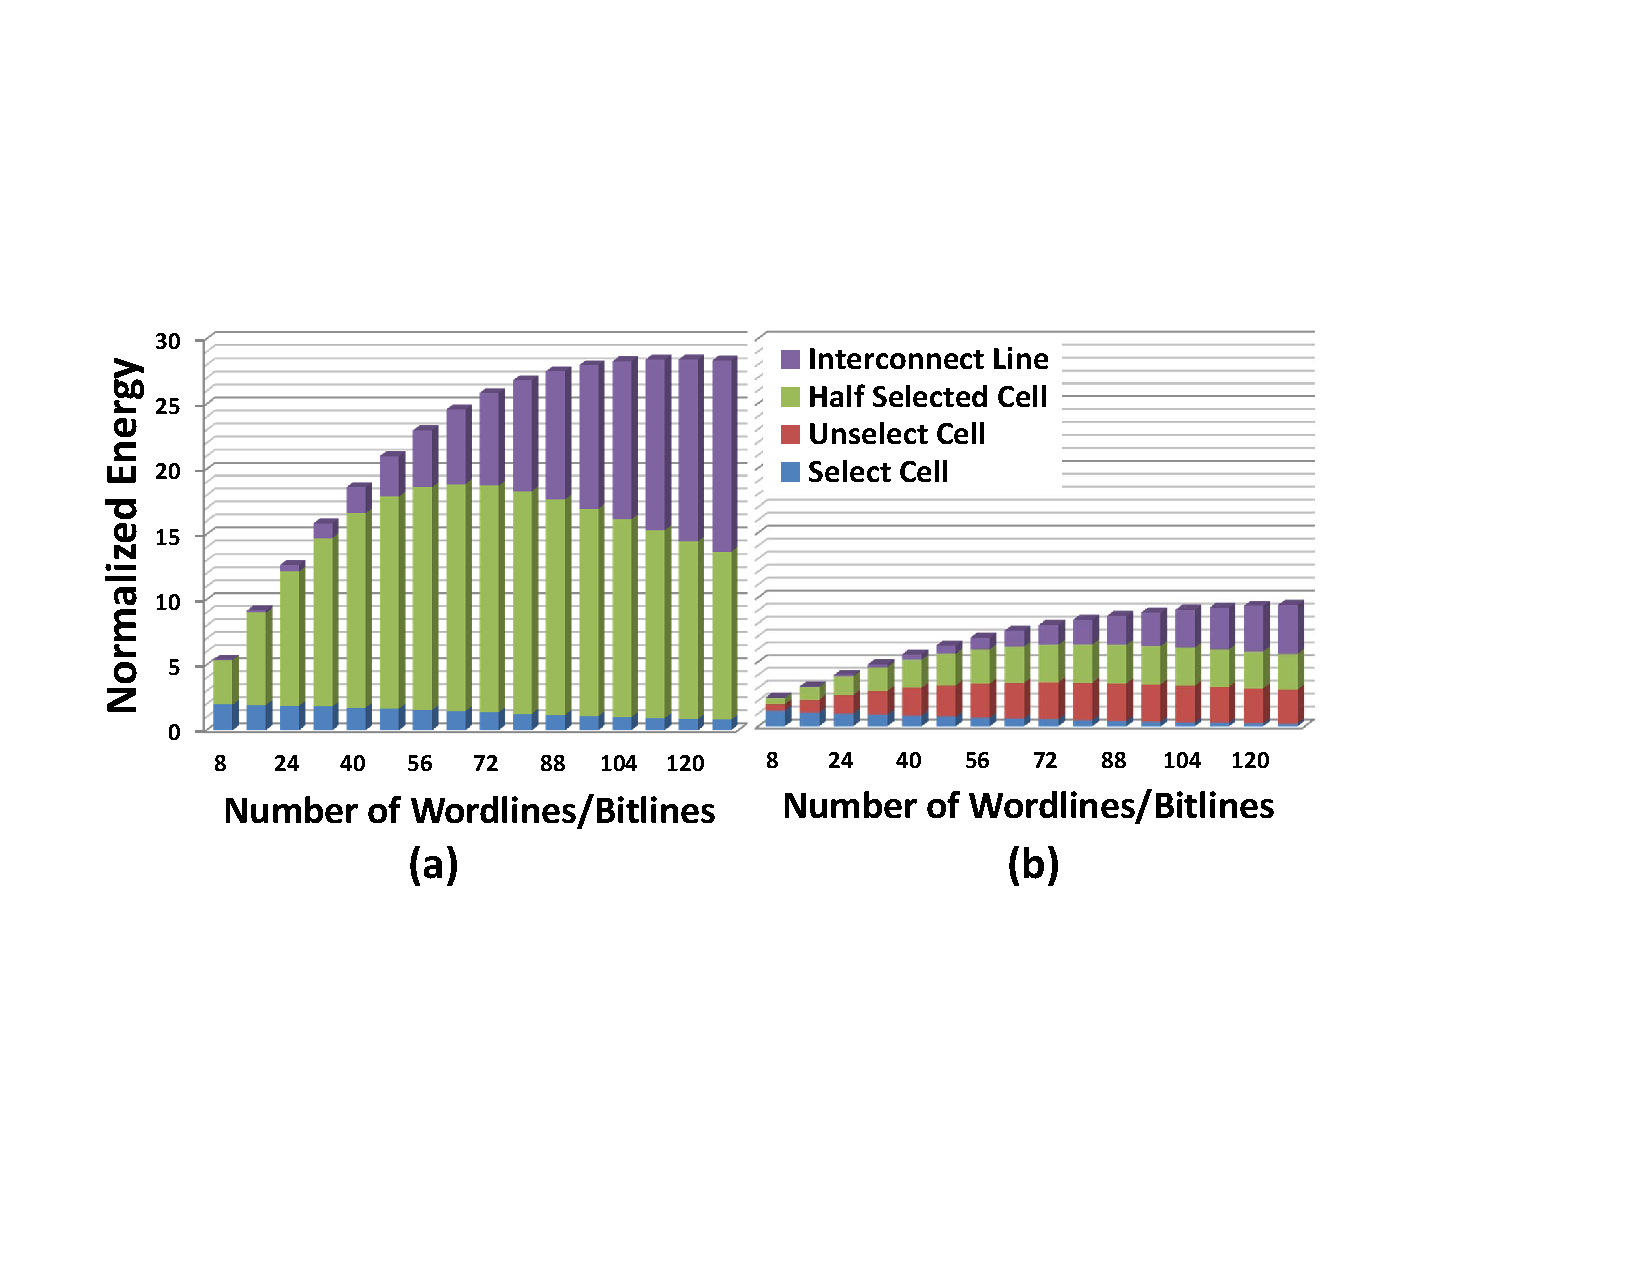
\includegraphics[width=0.5\textwidth]{./figures/multi_energy_f.pdf}\\
  \caption{The normalized energy consumption per bit for multi-bits write operation. (a): HWHB and  FWHB schemes; (b): HWFB scheme. }\label{fig:multi_energy}
    \vspace{-10pt}
\end{figure}



%\begin{figure}%[!t]
%\centering
%  % Requires \usepackage{graphicx}
%  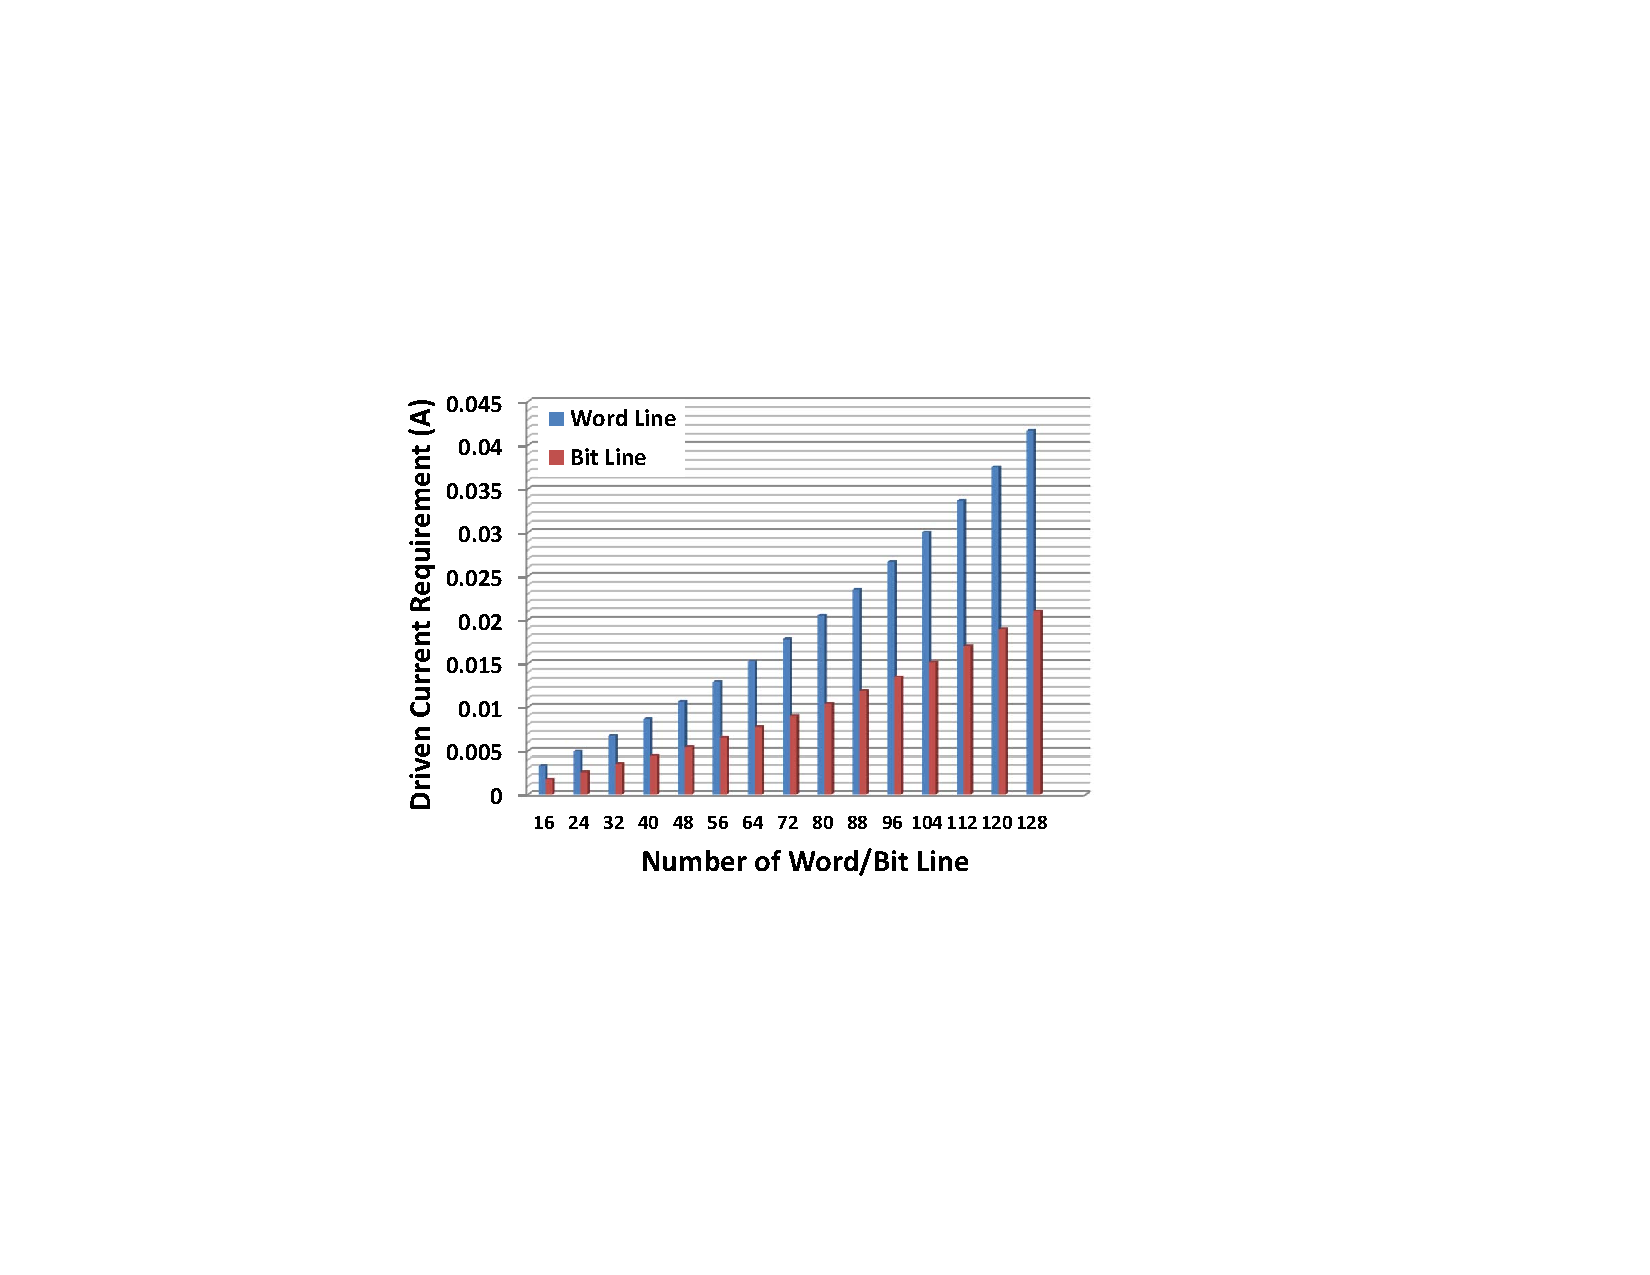
\includegraphics[width=0.4\textwidth]{./figures/multi_I2.pdf}\\
%  \caption{The }\label{fig:multi_I}
%\end{figure}

\vspace{6pt} \emph{Non-linearity of the ReRAM Cell.} \vspace{6pt}

\begin{figure}[!b]
\centering
  % Requires \usepackage{graphicx}
  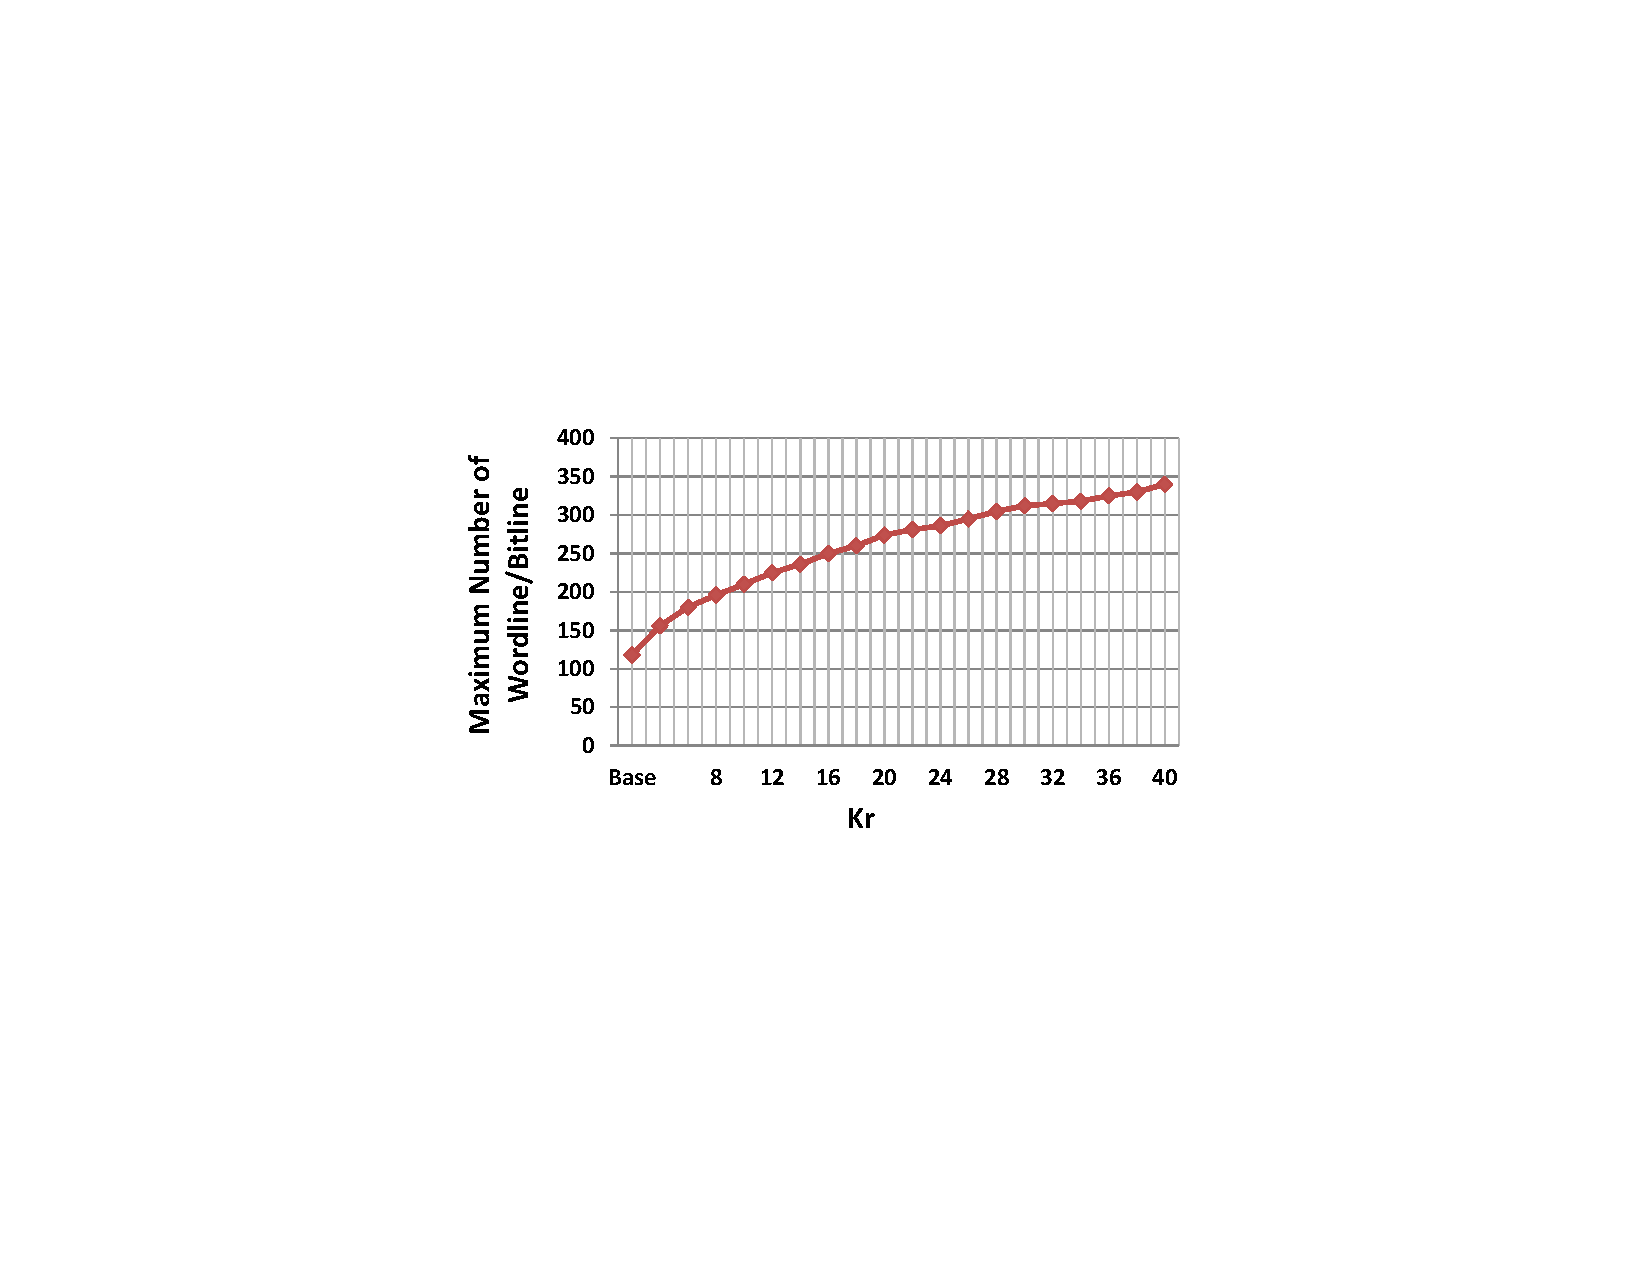
\includegraphics[width=0.4\textwidth]{./figures/non_linear_f}\\
  \caption{The maximum array size with different non-linearity coefficient.}\label{fig:non_linear}
\end{figure}
One of the most distinct features of ReRAM is its non-linearity. For example, the non-linearity of memristor-based ReRAM is observed at LRS when the resistance of the memristor cell is not constant but varies with the applied voltage. The non-linearity coefficient is defined as:
$K_r(p,V) = p \times R(V/p)/R(V)$, where $R(V/p)$ and $R(V)$ are the equivalent resistance of the memristor biased at $V/p$ and $V$~\cite{memristor:Cong}. Normally, the $K_r(p,V)$ value for memristor-based ReRAM is larger than 20, meaning that the resistance of a half-biased  cell is at least 10 times larger than a full-biased cell. Clearly, the ReRAM cell with a larger non-linearity coefficient results in a better memory cell since the current in the sneak path will be significantly reduced. In addition, the increased resistance at half-selected and unselected cells can also mitigate the voltage drop along the activated wordline and bitline. Figure~\ref{fig:non_linear} shows the influence of different non-linearity coefficients on the array size requirements for one bit HWHB writing scheme. In this figure, the maximum array size increases from $112 \times 112$ to $340 \times 340$ when the non-linearity coefficient $K_r$ increases from 1 to 10. Similarly, the non-linearity can also increase the maximum array size for other write schemes.


Moreover, the non-linearity can also reduce the energy consumption and area overheads of the cross-point array. For example, consider a $128 \times 128$ array. As shown in Figure~\ref{fig:non_linear_energy}, the energy consumption for the write operation decreases dramatically with the increase of non-linearity coefficient $K_r$. As $K_r$ increases from 1 to 40, the write energy is reduced by 98.3\%. The driven current requirement is shown in Figure~\ref{fig:area_all}(a), and the corresponding area overheads of the voltage drivers are compared to the array size at Figure~\ref{fig:area_all}(b). The baseline design is unacceptable because the area of voltage drivers is about 11.6 times larger than the area of the cross-point array. In this case, the area efficiency of ReRAM's $4F^2$ cell size will be offset by the extremely huge area overhead of the voltage drivers. However, with the increase of non-linearity, the area of voltage drivers becomes comparable to the array area. Therefore, we can conclude that, the ReRAM cells with a small non-linearity coefficient are not suitable for the cross-point structure based memory array. Next, we study the area overhead of multi bit write. Figure~\ref{fig:Area_kr20} shows the normalized areas of the voltage drivers for one bit and multi bit write operations. As mentioned, multi-bit write operations require larger driven current. Therefore, the area of voltage drivers for multi bit write operations are much larger than that for one bit write operations. Finally, normalized areas of the one bit and multi bit write operations have opposite trends as the array size increases. Normalized area for one bit write operation increases with the array size. On the contrary, normalized area for multi bit write decreases as the array size increase.

\begin{figure}%[!t]
\centering
  % Requires \usepackage{graphicx}
  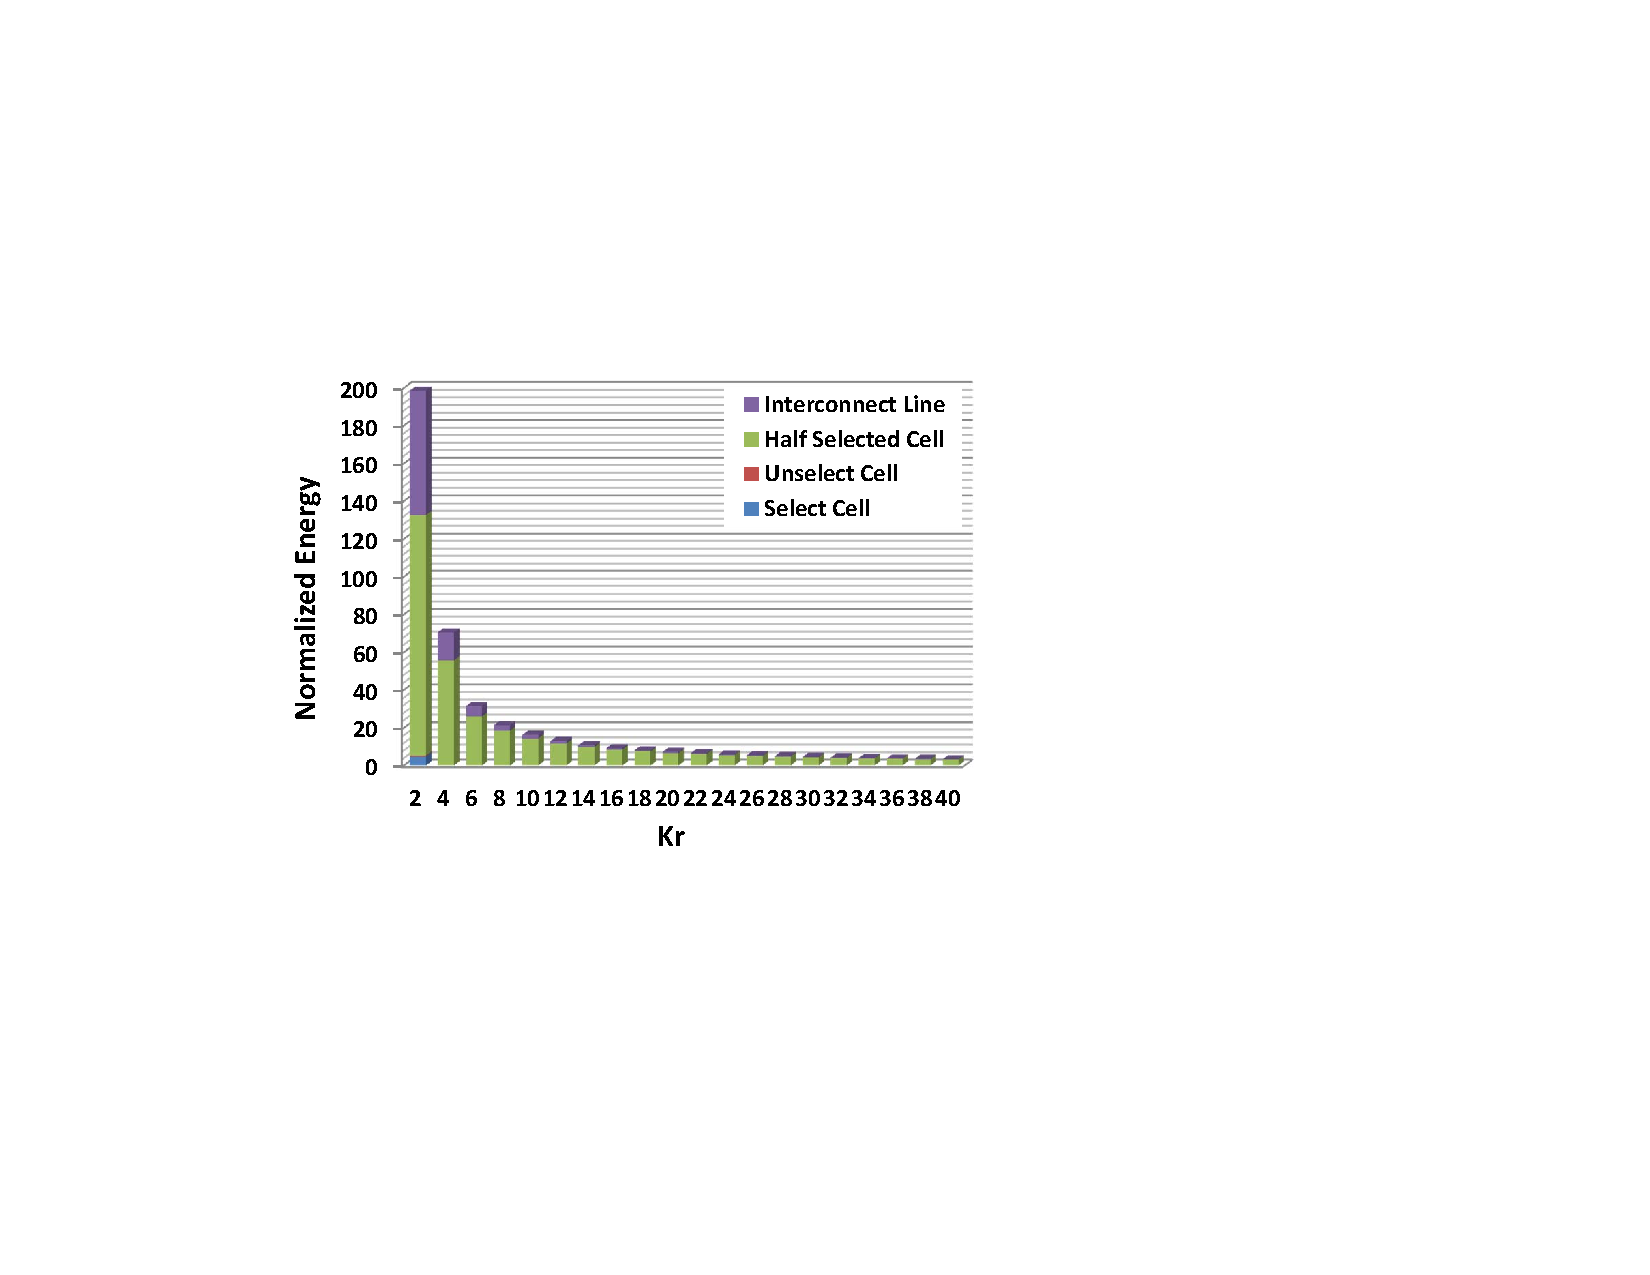
\includegraphics[width=0.38\textwidth]{./figures/non_linear_energy.pdf}\\
  \caption{The normalized energy consumption with non-linear ReRAM cells.}\label{fig:non_linear_energy}
\end{figure}

%\begin{figure}%[!t]
%\centering
%  % Requires \usepackage{graphicx}
%  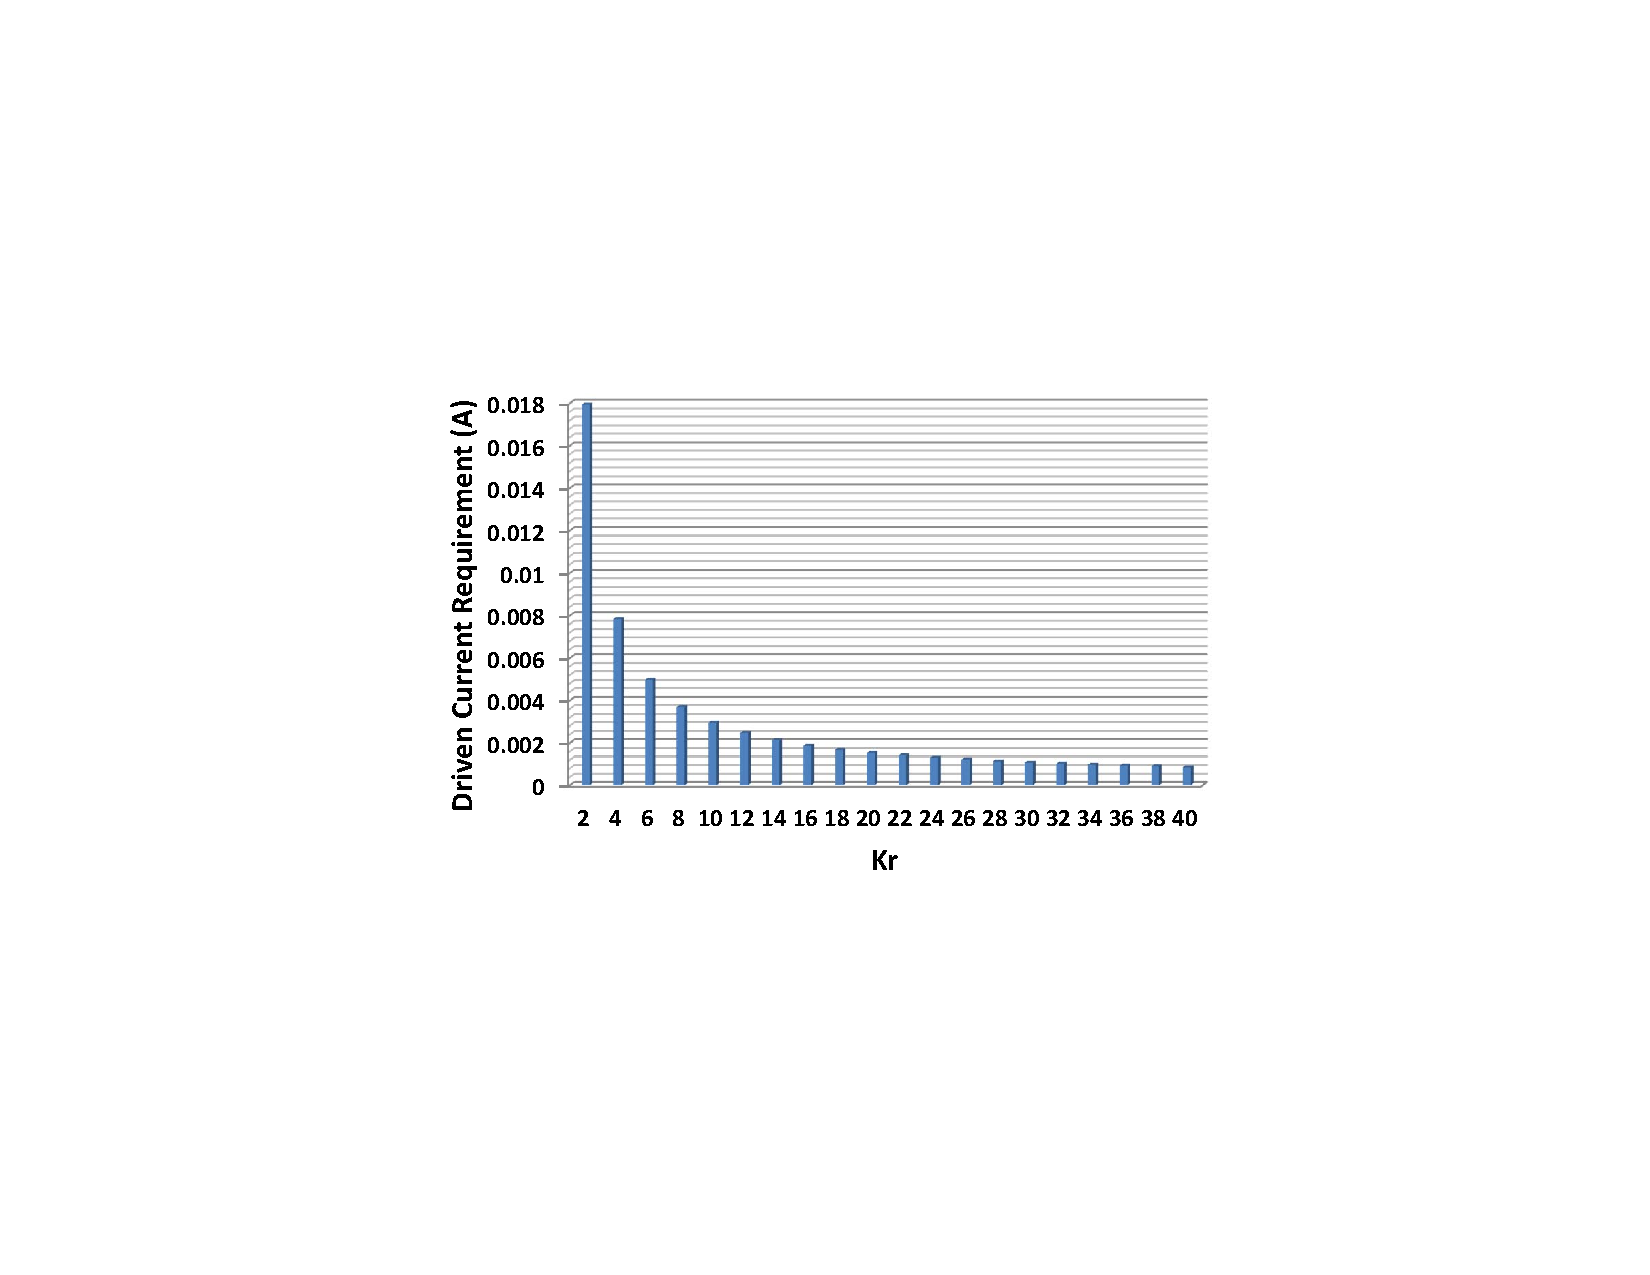
\includegraphics[width=0.4\textwidth]{./figures/non_linear_I.pdf}\\
%  \caption{The}\label{fig:non_linear_I}
%\end{figure}
%
%\begin{figure}%[!t]
%\centering
%  % Requires \usepackage{graphicx}
%  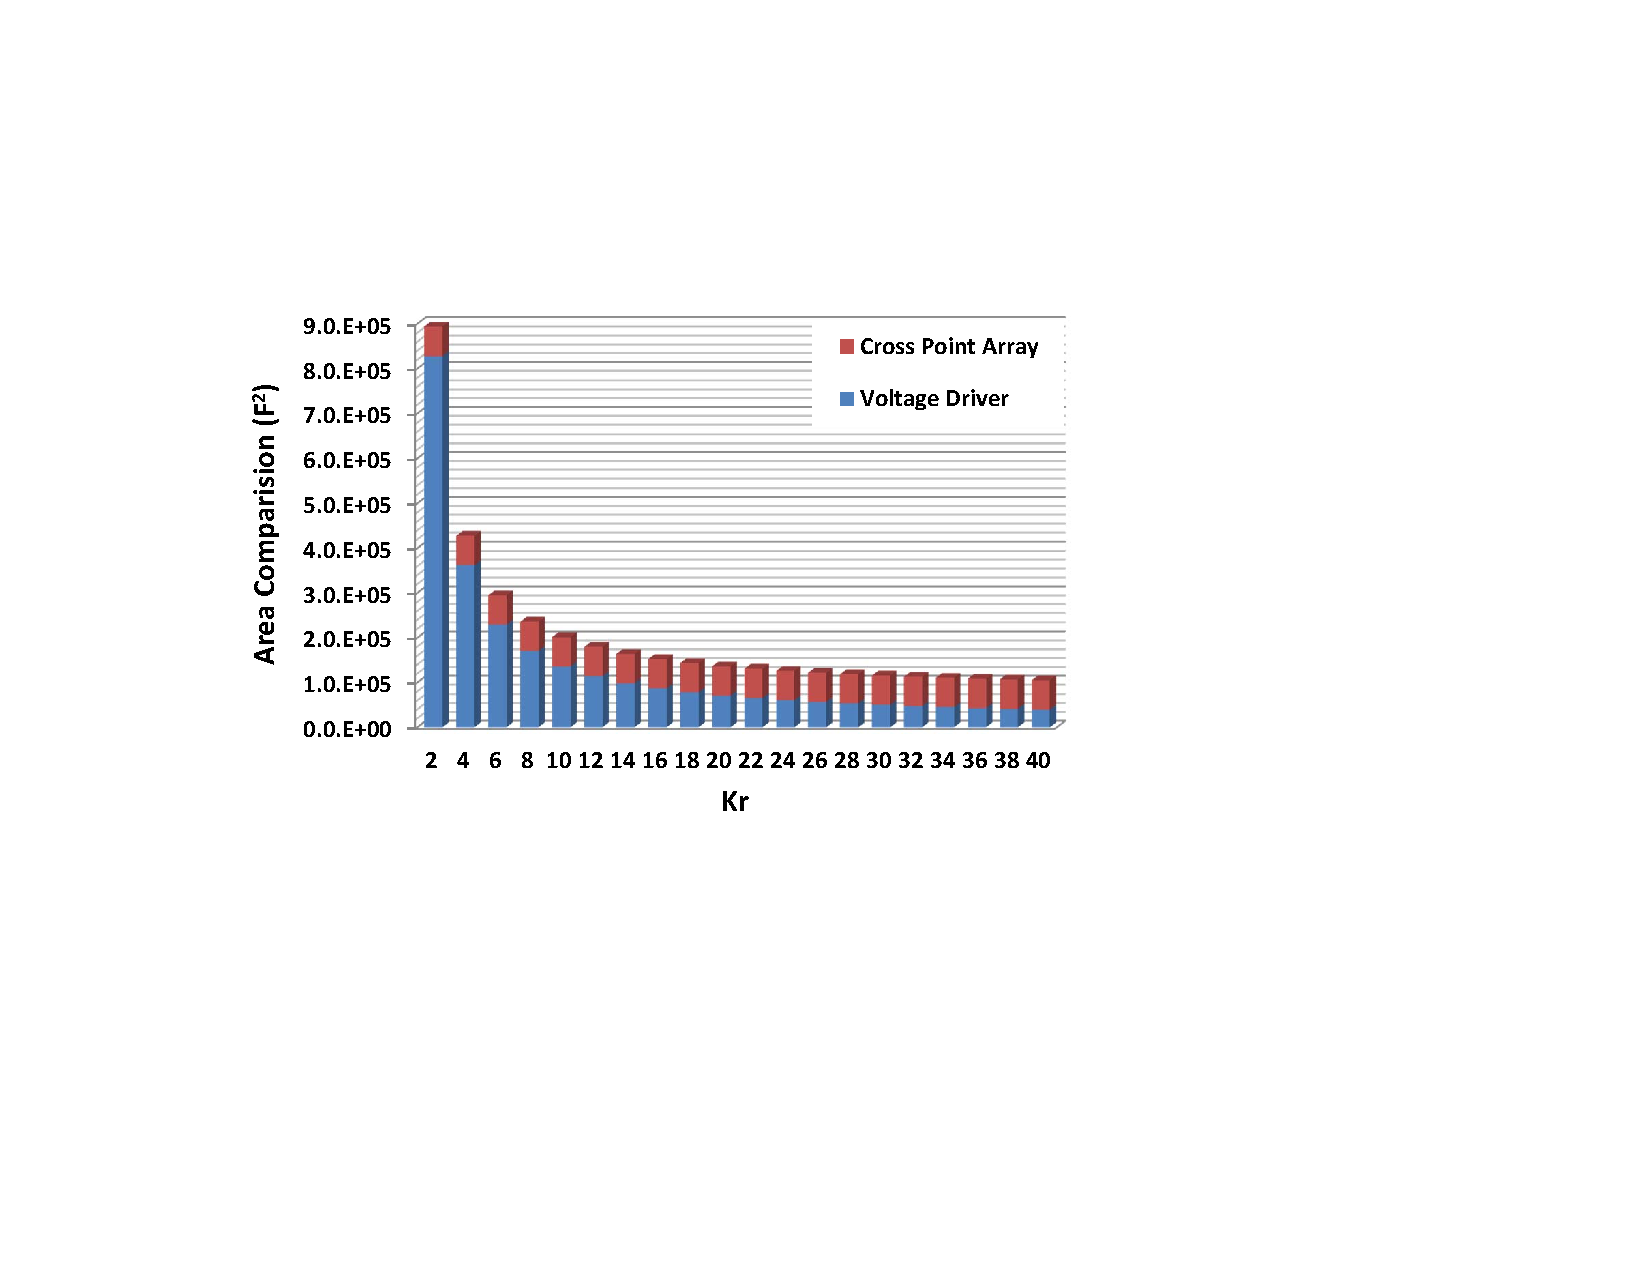
\includegraphics[width=0.4\textwidth]{./figures/non_linear_ara.pdf}\\
%  \caption{The}\label{fig:non_linear_ara}
%\end{figure}
\begin{figure}%[!t]
\centering
  % Requires \usepackage{graphicx}
  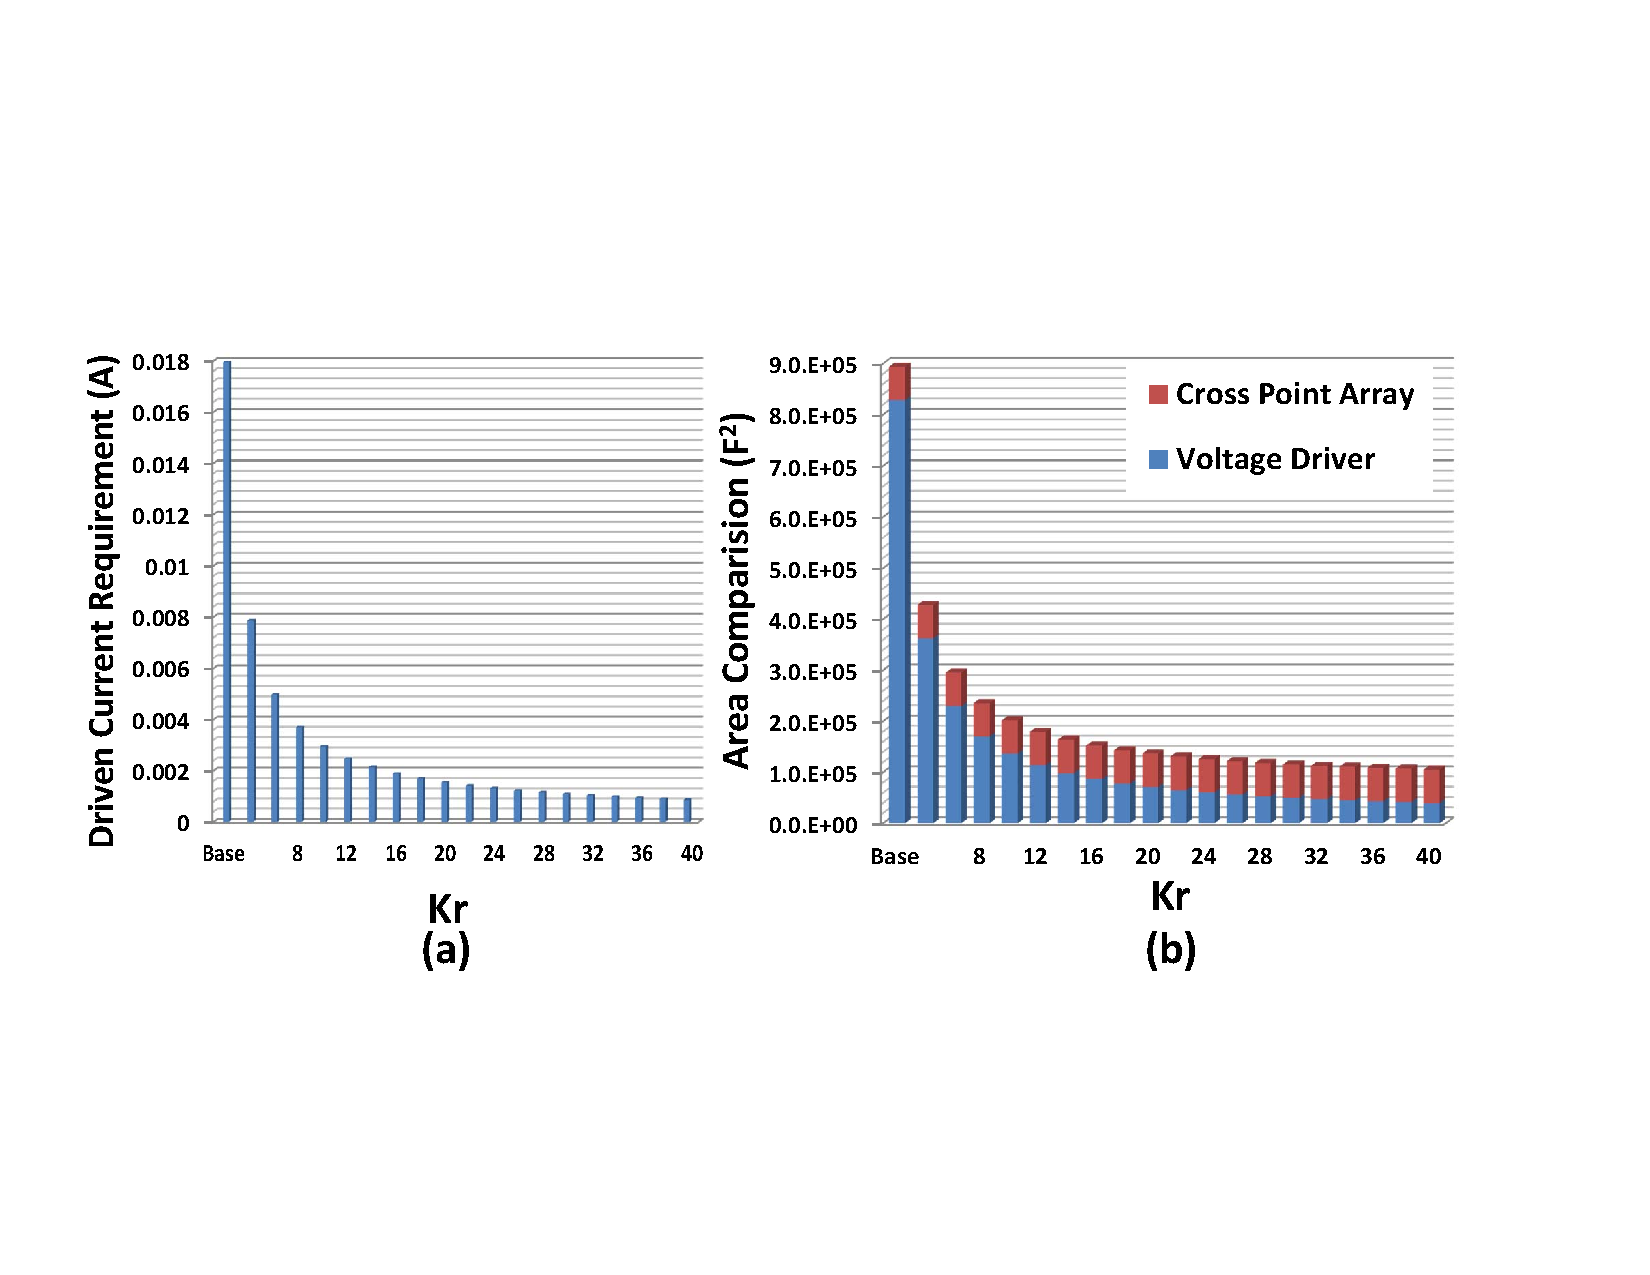
\includegraphics[width=0.5\textwidth]{./figures/area_all.pdf}\\
  \vspace{-5pt}
  \caption{The driven current requirements and area overheads with different non-linearity coefficients}\label{fig:area_all}
 \vspace{-15pt}
\end{figure}


\begin{figure}%[!t]
\centering
  % Requires \usepackage{graphicx}
  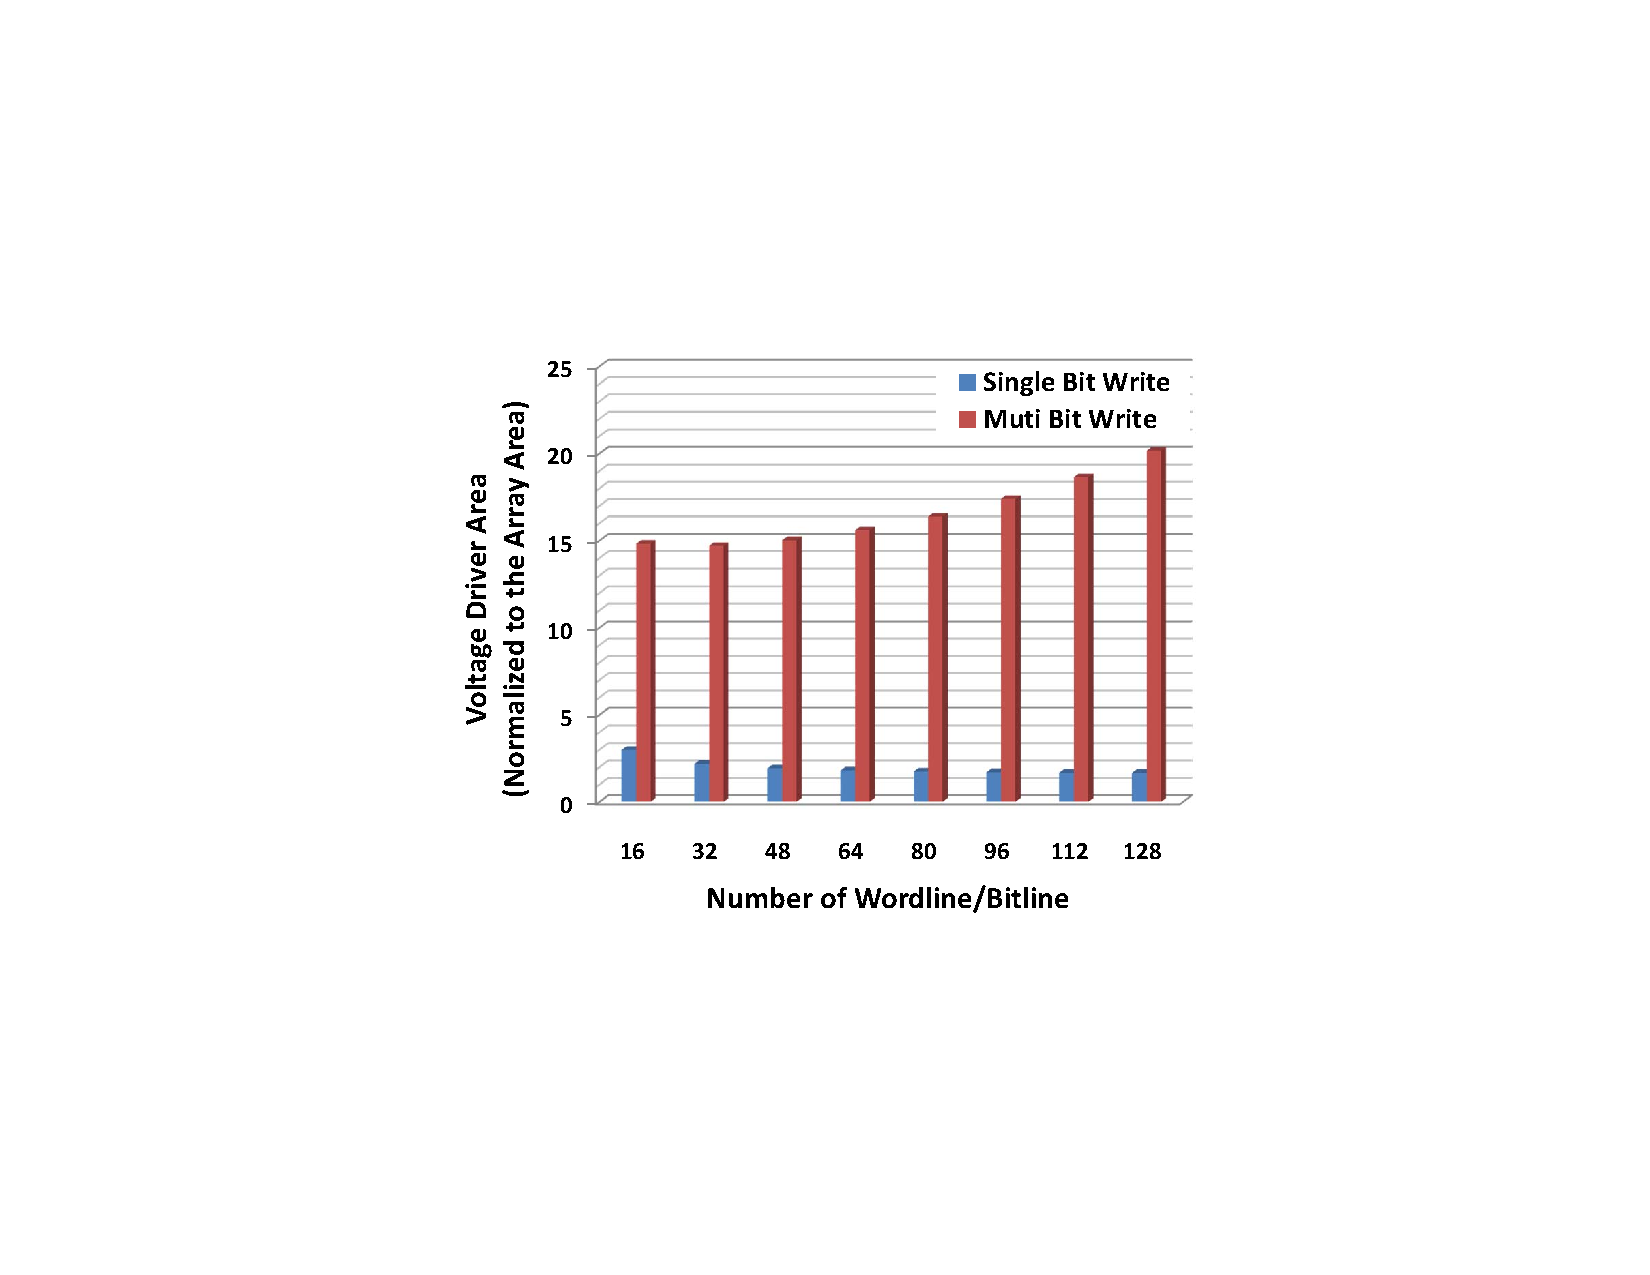
\includegraphics[width=0.35\textwidth]{./figures/Area_kr20_f.pdf}\\
  \caption{The normalized area overhead of voltage drivers ($K_r=20$, the areas are normalized to the area of cross-point array). }\label{fig:Area_kr20}
\end{figure}
\subsection{Read Operation}
In this section, the current sensing scheme is used to determine the current in each bitline. In order to read cell $R_{i,j}$, the $i^{th}$ wordline is biased at $V_{READ}$ and all of the other wordlines and bitlines are grounded. Then the state of the selected cell is read out by measuring the voltage across $R_s$. The energy consumption for read operation can be analyzed by the same way as that of the write operation. Considering the read voltage is much smaller than write voltage, the read energy is expected at least one order smaller than write operation. Besides, since the read voltage/current is much lower than the write, we believe that the voltage drivers can always provide enough current for the read operation if they meet the current requirement for write operation. Therefore, we can conclude that the area overhead of voltage drivers is determined by the write current. However, the reliability of read operation is different from the write operation. The read reliability is determined by the voltage swing for reading HRS and LRS cells. Figure~\ref{fig:sense_margin} (a) shows the voltage swing with different array sizes and $K_r$ values. Large array sizes and large non-linearity are harmful to the voltage swing: on the one hand, larger array has more sneak paths,making the output voltage very sensitive to the data pattern of unselected cells; on the other hand, the non-linearity increases the resistance of LRS and therefore reduces the ON-OFF resistance ratio. In order to improve the reliability of the read operation, a two-step sensing scheme can be applied, which senses the current of unselected cell first, then the overall current is sensed, and after that the current difference is converted to the output voltage. The voltage swing of this two-step sensing scheme is shown in Figure~\ref{fig:sense_margin} (b). By using the two steps sensing schemes, the voltage swing is doubled for the array with same size and non-linearity coefficient.

%\begin{figure}%[!t]
%\centering
%  % Requires \usepackage{graphicx}
%  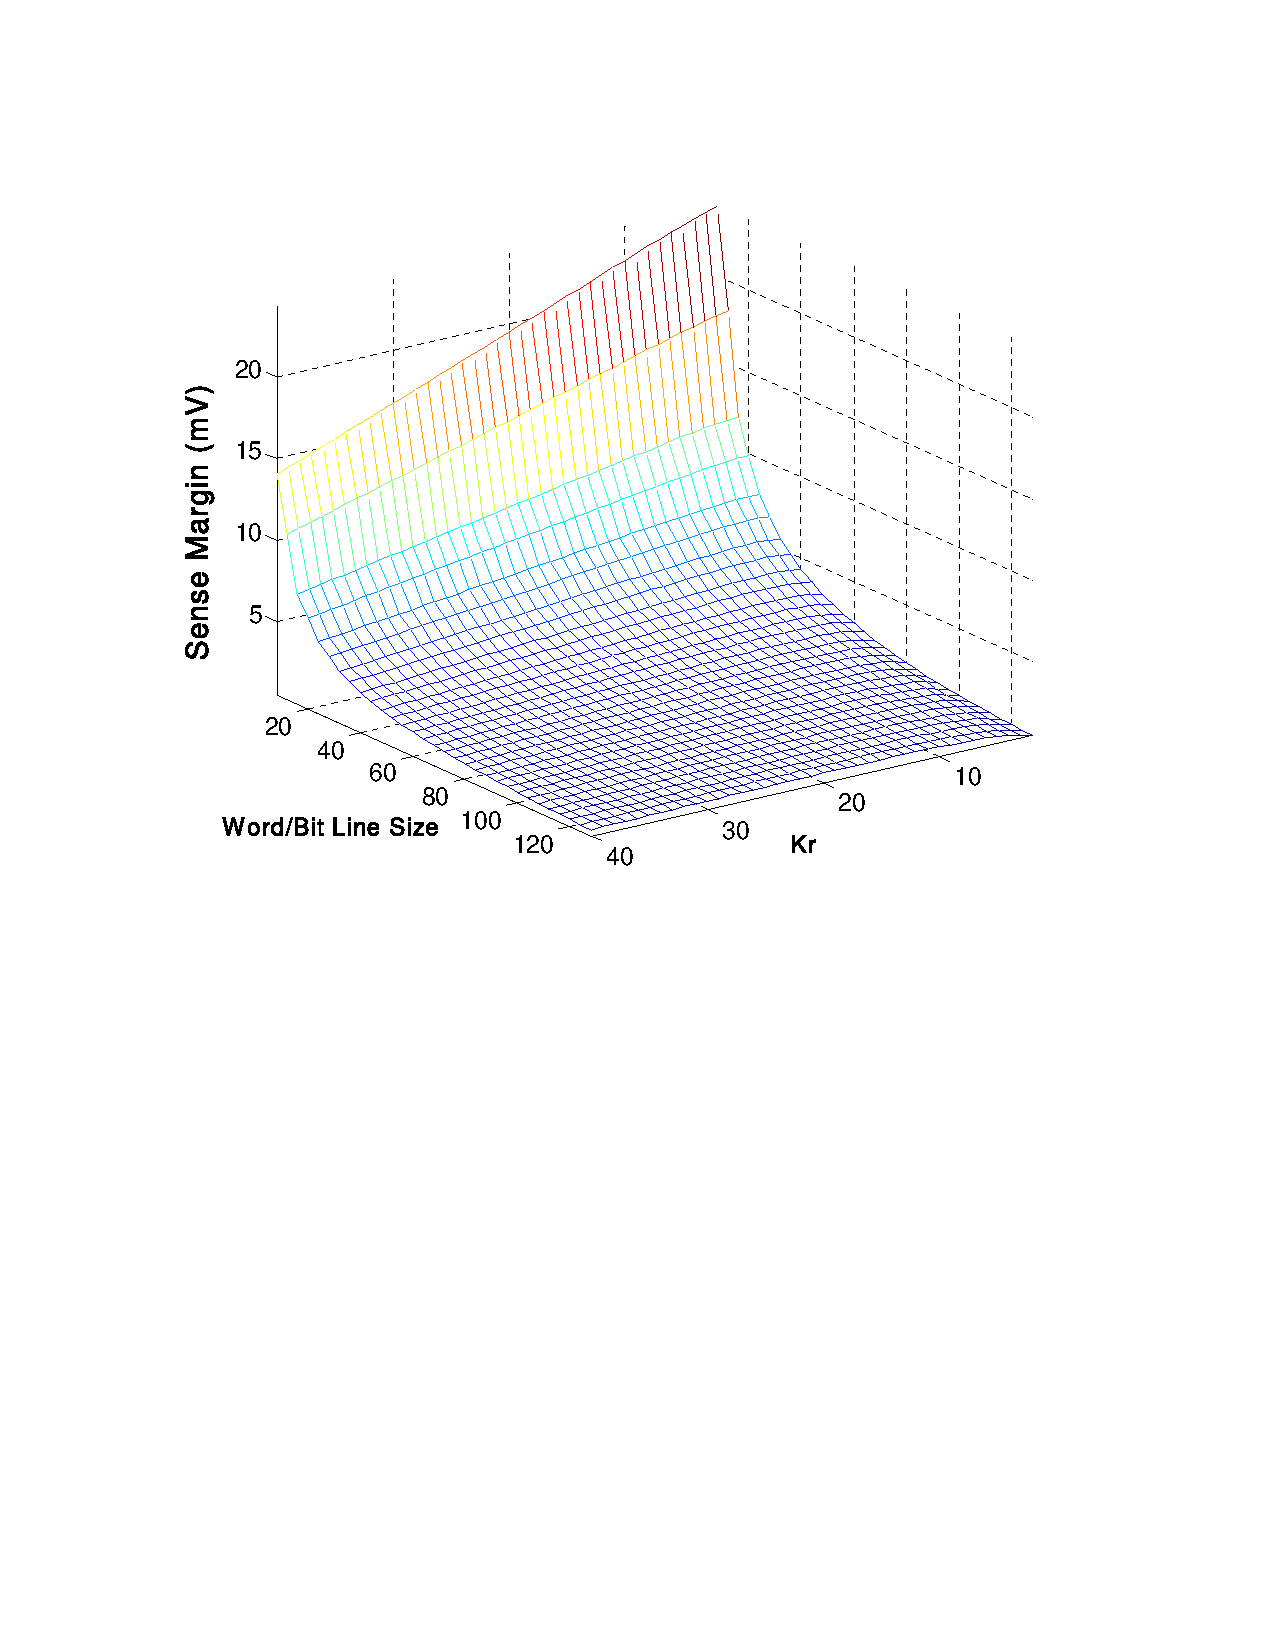
\includegraphics[width=0.45\textwidth]{./figures/margin.pdf}
%  \caption{The}\label{fig:margin}
%\end{figure}
%
%\begin{figure}%[!t]
%\centering
%  % Requires \usepackage{graphicx}
%  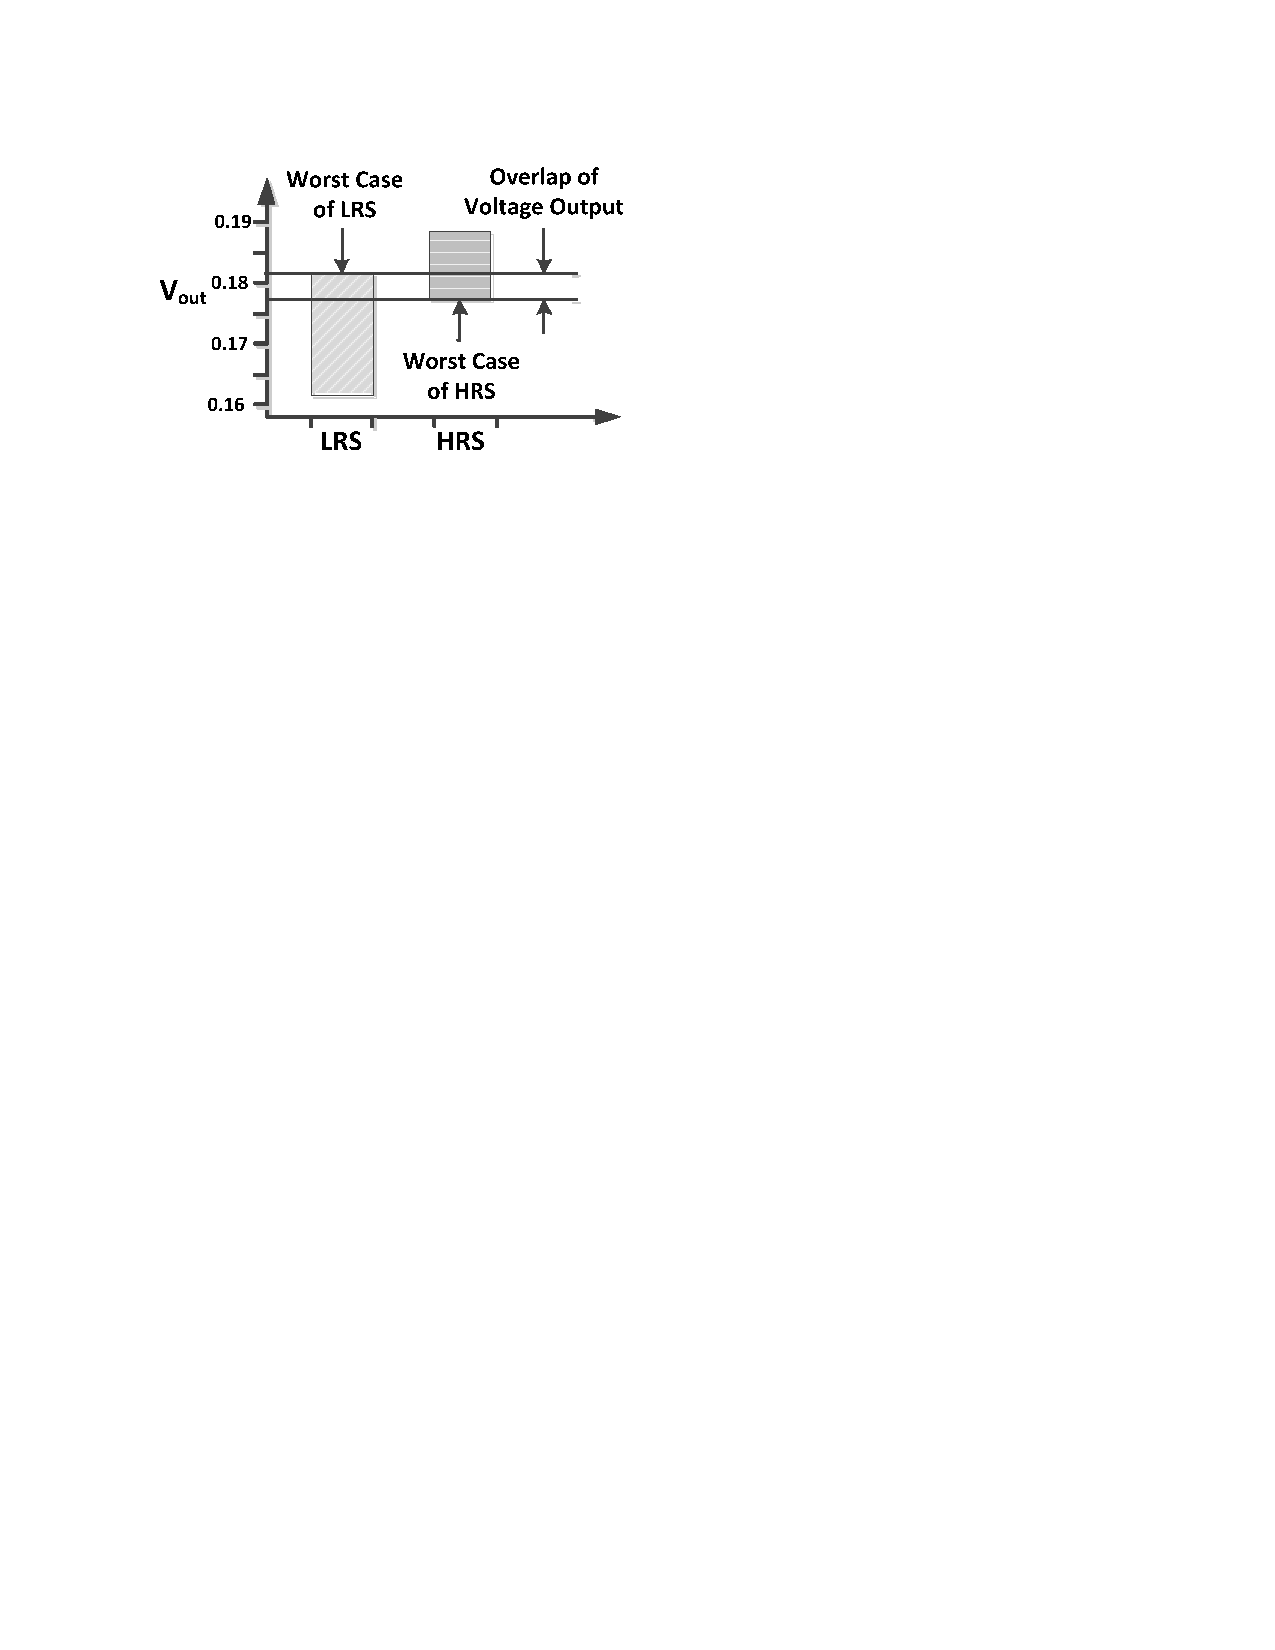
\includegraphics[width=0.4\textwidth]{./figures/overlap.pdf}\\
%  \caption{The}\label{fig:overlap}
%\end{figure}

%
%\begin{figure}%[!t]
%\centering
%  % Requires \usepackage{graphicx}
%  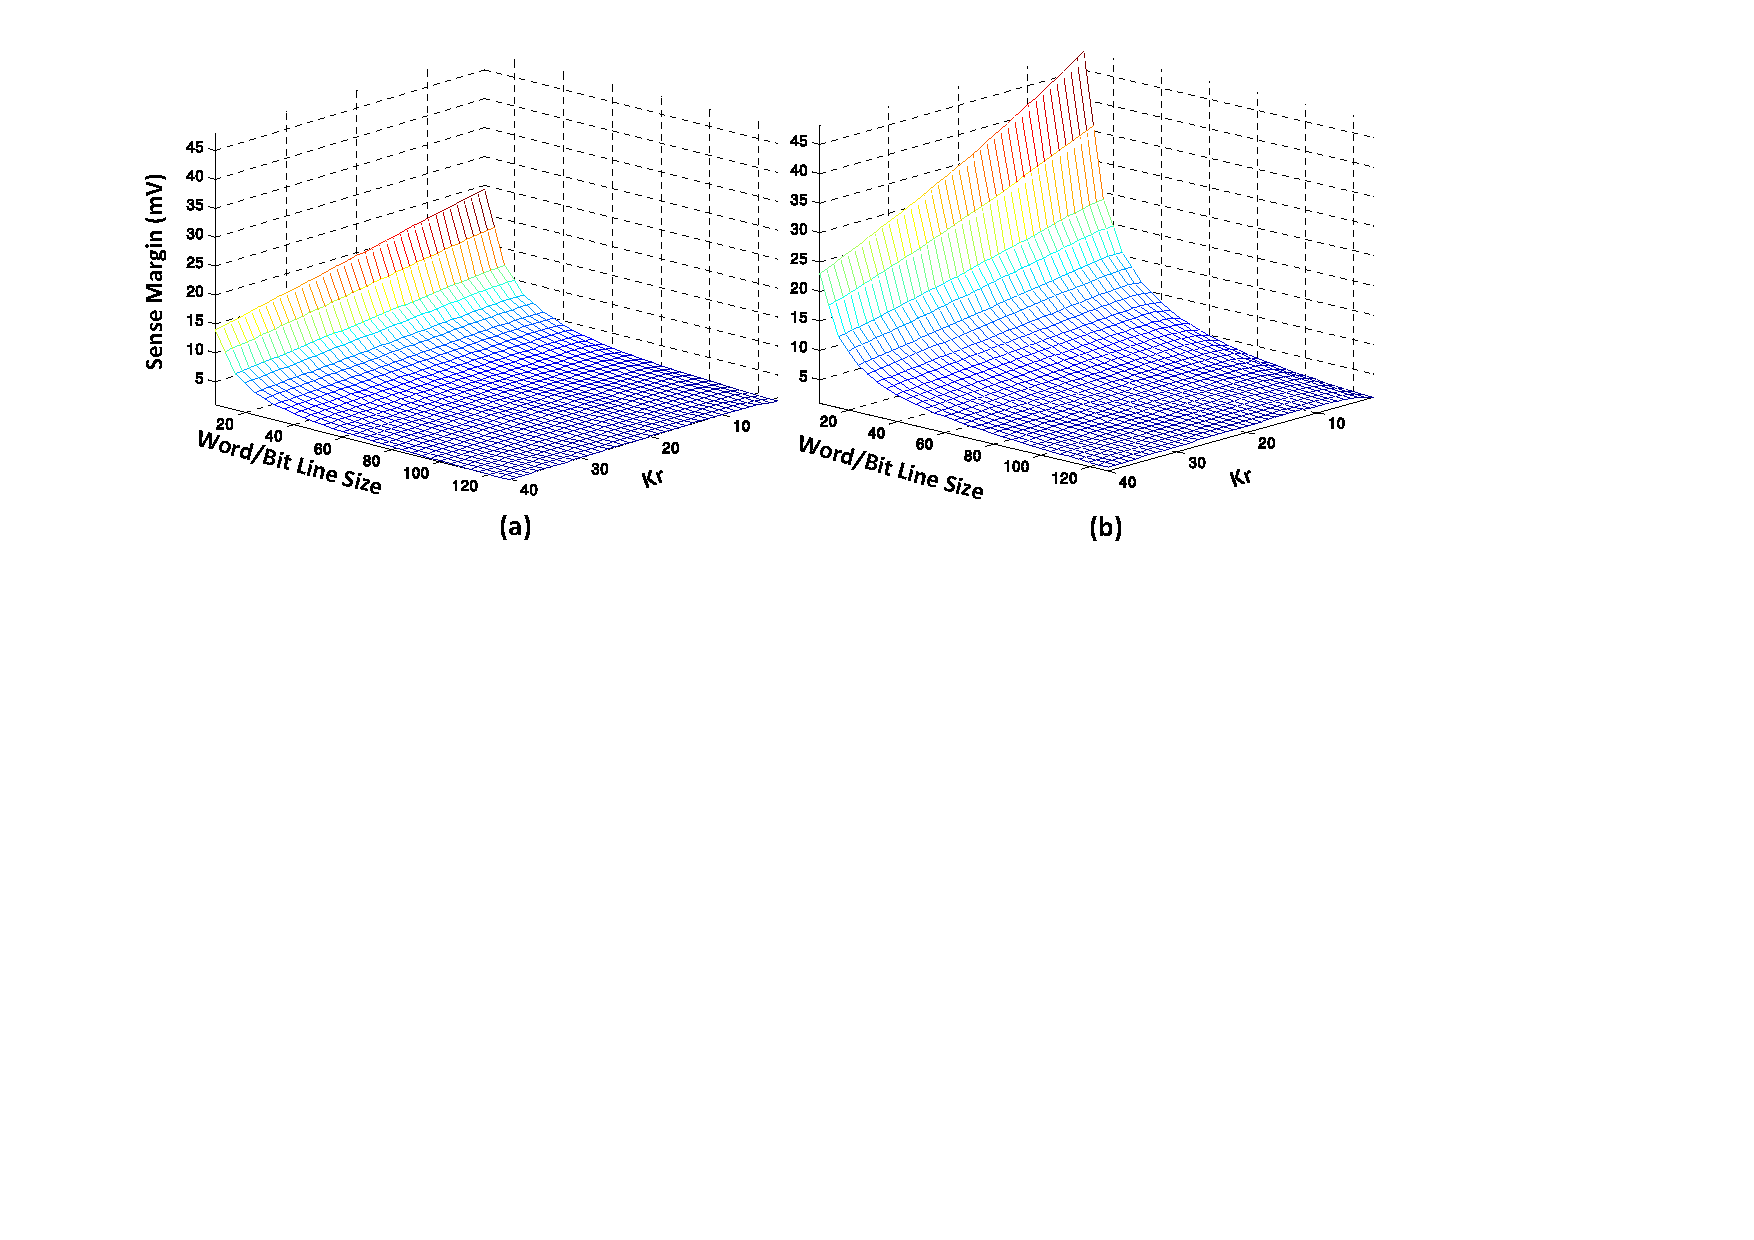
\includegraphics[width=0.5\textwidth]{./figures/sense_margin21}\\
%  \caption{The}\label{fig:sense_margin}
%\end{figure}

\begin{figure}[!b]
\centering
  % Requires \usepackage{graphicx}
  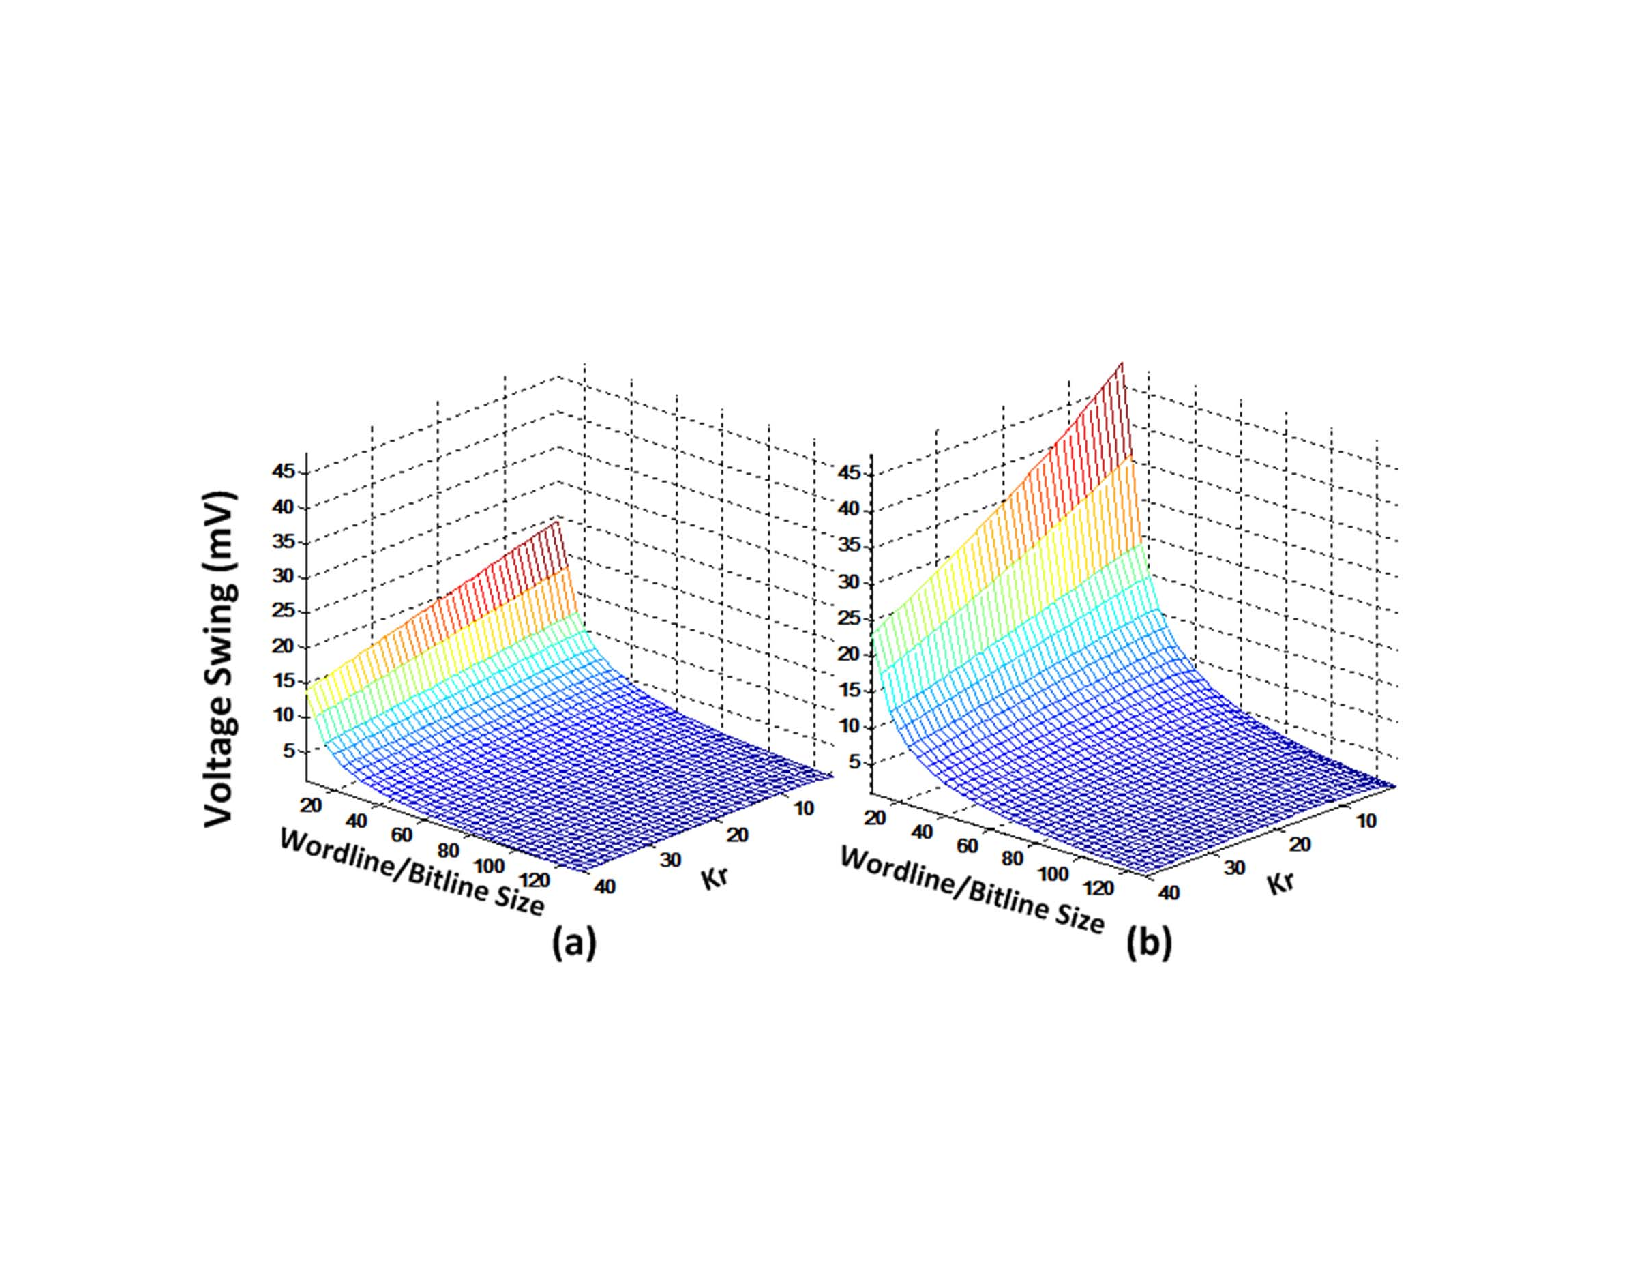
\includegraphics[width=0.5\textwidth]{./figures/sense_margin_f}\\
  \caption{Relationships among the voltage swing, array size and non-linearity. (a) Normal sensing scheme; (b) Two-step sensing scheme}\label{fig:sense_margin}
\end{figure}
